\documentclass[
	% -- opções da classe memoir --
	12pt,				% tamanho da fonte
	openright,			% capítulos começam em pág ímpar (insere página vazia caso preciso)
	twoside,			% para impressão em verso e anverso. Oposto a oneside
	a4paper,			% tamanho do papel. 
	% -- opções da classe abntex2 --
	%chapter=TITLE,		% títulos de capítulos convertidos em letras maiúsculas
	%section=TITLE,		% títulos de seções convertidos em letras maiúsculas
	%subsection=TITLE,	% títulos de subseções convertidos em letras maiúsculas
	%subsubsection=TITLE,% títulos de subsubseções convertidos em letras maiúsculas
	% -- opções do pacote babel --
	english,			% idioma adicional para hifenização			
	brazil				% o último idioma é o principal do documento
	]{abntex2}

% ---
% Pacotes básicos 
% ---
\usepackage{lmodern}
\usepackage{lastpage}			% Usado pela Ficha catalográfica
\usepackage{indentfirst}		% Indenta o primeiro parágrafo de cada seção.
\usepackage[utf8]{inputenc}
\usepackage[T1]{fontenc}
\usepackage[brazilian,hyperpageref]{backref}	 % Paginas com as citações na bibl
\usepackage[alf]{abntex2cite}	% Citações padrão ABNT
\usepackage{microtype} 			% para melhorias de justificação

% \usepackage[fixlanguage]{babelbib}
\usepackage{amsmath}
\usepackage[colorinlistoftodos]{todonotes}
\usepackage{tabularx}
\usepackage{multirow}
\usepackage{graphicx}
\usepackage{listings}
\usepackage{url}
\usepackage{float}
\usepackage{comment}
\usepackage{caption}
\usepackage{color}
%\usepackage{nomencl}
%\usepackage{fontspec}
%\usepackage{titlesec}
\definecolor{lightgray}{rgb}{0.95,0.95,0.95}
\linespread{1.25}

% --- 
% CONFIGURAÇÕES DE PACOTES
% --- 

% ---
% Configurações do pacote backref
% Usado sem a opção hyperpageref de backref
%\renewcommand{\backrefpagesname}{Citado na(s) página(s):~}
% Texto padrão antes do número das páginas
%\renewcommand{\backref}{}
% Define os textos da citação
%\renewcommand*{\backrefalt}[4]{
%	\ifcase \#1 %
%		Nenhuma citação no texto.%
%	\or
%		Citado na página \#2.%
%	\else
%		Citado \#1 vezes nas páginas \#2.%
%	\fi}%
% ---

% ---
% Informações de dados para CAPA e FOLHA DE ROSTO
% ---
\titulo{Sistema de Monitoramento Residencial de Uso de Energia}
\autor{Henrique Sussumu Matsui Kano \& Mi Che Li Lee}
\local{São Paulo}
\date{2015}
\orientador{Professor Doutor Carlos Eduardo Cugnasca}
\instituicao{%
  Escola Politécnica da Universidade de São Paulo
  \par
  Departamento de Computação e Sistemas Digitais
  \par
  Graduação}
\tipotrabalho{Dissertação (Graduação)}
% O preambulo deve conter o tipo do trabalho, o objetivo, 
% o nome da instituição e a área de concentração 
\preambulo{Dissertação apresentada à Escola Politécnica da Universidade de São Paulo para a conclusão do curso de graduação em Engenharia de Computação}
% ---

% ---
% Configurações de aparência do PDF final

% alterando o aspecto da cor azul
\definecolor{blue}{RGB}{41,5,195}

% informações do PDF
\makeatletter
\hypersetup{
     	%pagebackref=true,
		pdftitle={\@title}, 
		pdfauthor={\@author},
    	pdfsubject={\imprimirpreambulo},
	    pdfcreator={LaTeX with abnTeX2},
		pdfkeywords={abnt}{latex}{abntex}{abntex2}{trabalho acadêmico}, 
		colorlinks=true,       		% false: boxed links; true: colored links
    	linkcolor=blue,          	% color of internal links
    	citecolor=blue,        		% color of links to bibliography
    	filecolor=magenta,      		% color of file links
		urlcolor=blue,
		bookmarksdepth=4
}
\makeatother
% --- 

% --- 
% Espaçamentos entre linhas e parágrafos 
% --- 

% O tamanho do parágrafo é dado por:
\setlength{\parindent}{1.3cm}

% Controle do espaçamento entre um parágrafo e outro:
\setlength{\parskip}{0.2cm}  % tente também \onelineskip

% ---
% compila o indice
% ---
\makeindex
% ---


\lstset{%
  backgroundcolor=\color{lightgray},
  commentstyle=\color{gray},
  basicstyle=\footnotesize\ttfamily,
  breaklines=true, 
  tabsize=2,
  captionpos=b
}
\makenomenclature
\begin{document}
\begin{titlepage}

\begin{center}
\vspace{30mm}
\large
Escola Politécnica da Universidade de São Paulo\\
Henrique Sussumu Matsui Kano\\
Mi Che Li Lee

\vspace{90mm}
\Large
Sistema de Monitoramento Residencial de Uso de Energia

\vfill
São Paulo\\
2015

\end{center}

\end{titlepage}

\begin{titlepage}

\begin{center}

\small


\vfill

\LARGE

\textbf{Sistema de Monitoramento Residencial\\ 
de Uso de Energia}

\vfill

\large

\textbf{Henrique Sussumu Matsui Kano}

\textbf{Mi Che Li Lee}

\vfill

\normalsize

Orientador: Prof. Dr. Carlos Cugnasca

\vfill

\vfill

\large

%Data
Maio de 2015

\end{center}

\end{titlepage}
\begin{fichacatalografica}
	\vspace*{\fill}					% Posição vertical
	\begin{center}
		Catalogação-na-publicação
	\end{center}
	\hrule							% Linha horizontal
	\begin{center}					% Minipage Centralizado
	\begin{minipage}[c]{12.5cm}		% Largura
	
	Kano, Henrique 
	
	\hspace{0.5cm} Sistema de monitoramento residencial de uso de energia / H. Kano, M. Lee -- São Paulo, 2015.
	
	\hspace{0.5cm} \pageref{LastPage} p.\\
	
	\hspace{0.5cm}
	\parbox[t]{\textwidth}{Trabalho de Formatura - Escola Politécnica da Universidade de São
Paulo. Departamento de Engenharia de Computação e Sistemas Digitais.}\\
	\\
	
	\hspace{0.5cm}
		1. SENSOR.
		2. COMPUTAÇÃO MÓVEL.
		3. CONSUMO DE ENERGIA ELÉTRICA.
		4. INTERNET.
		I. Universidade de São Paulo. Escola Politécnica. Departamento de Engenharia de Computação e Sistemas Digitais
		II. t.
		III. Lee, Mi\\ 			
	
	\end{minipage}
	\end{center}
	\hrule
\end{fichacatalografica}
% ---

%\begin{fichacatalografica}
%    \includepdf{Anexos/EPUSP-Catalogacao-na-Fonte.pdf}
%\end{fichacatalografica}
\begin{agradecimentos}
\vspace{10mm}
Agradeço minha família pelo suporte emocional.

Ao professor orientador pela orientação e dedicação constante ao trabalho.

Aos técnicos Fátima, Daniel do labdigi e Marcelo do labmicro pelo suporte técnico dado.

Ao pessoal da DevTecnologia pela orientação inicial.

Aos meus amigos que sempre deram o suporte nas horas difíceis.

\vspace{10mm}
Henrique Sussumu Matsui Kano 
\vspace{40mm}

Enfim, a jornada foi longa e sem ajuda eu não teria chegado até aqui. Por isso eu quero dizer que estou muito grata por tudo que aconteceu, seja fácil ou difícil. Eu sou grata pelas minhas amizades formadas desde o primeiro ano da Poli. Quero agradecer pelo constante apoio da mínha família. Admiro a paciência dos técnicos dos laboratórios do PCS. Sou grata pelo nosso orientador e por todos os nossos professores, por compartilhar suas experiências, nos ajudando da melhor forma possível. E sou muitíssimo grata pela minha igreja e a Deus, por ter me provido tudo que eu precisava.

\vspace{10mm}
Mi Che Li Lee
\hfill
\end{agradecimentos}


\setlength{\absparsep}{18pt} % ajusta o espaçamento dos parágrafos do resumo
\begin{resumo}

 O trabalho descreve a construção de um sistema de monitoramento de consumo de energia em uma residência. O sistema é composto por dispositivos interligados por uma rede sem fio e uma aplicação Web. O trabalho também funciona com o uso de serviços, recursos e ferramentas gratuitos para o desenvolvimento de uma interface gráfica para visualização dos dados de consumo.

 \textbf{Palavras-chaves}: IoT. Rede de Sensores sem fio. Computação em nuvem. Consumo de Energia Elétrica.
\end{resumo}

\begin{resumo}[Abstract]
 \begin{otherlanguage*}{english}
   This work describes one way to build a system for residence energy consumption monitoring with a low investment. The proposed system uses services, resources and tools that converges to a user friendly interface so that data collected may be easily analyzed by the user and system resources distribution organized by this interface.

   \vspace{\onelineskip}
 
   \noindent 
   \textbf{Key-words}: IoT. Wireless Sensor Network. Cloud Computing. Electric Power Consumption.
 \end{otherlanguage*}
\end{resumo}

\frontmatter
\addcontentsline{toc}{chapter}{Sumário}   
\tableofcontents

\cleardoublepage 
\addcontentsline{toc}{chapter}{Lista de Figuras}  
\listoffigures  

\cleardoublepage 
\addcontentsline{toc}{chapter}{Lista de Tabelas} 
\listoftables  

\cleardoublepage 
\addcontentsline{toc}{chapter}{Lista de Codigos}
\lstlistoflistings

\begin{simbolos}
  \item[$ \Gamma $] Letra grega Gama
  \item[$ \Lambda $] Lambda
  \item[$ \zeta $] Letra grega minúscula zeta
  \item[$ \in $] Pertence
\end{simbolos}


\mainmatter

\pagestyle{headings}

\chapter{Introdução}
\label{Cap:Introducao}

\section{Objetivo}
\label{Sec:objetivo}

O trabalho descreve a construção de um sistema para monitorar o uso de energia dentro da residência. O sistema consiste de dispositivos interligados por uma rede sem fio, composta por: uma rede local de sensores  que fará o sensoriamento dos parâmetros e se comunicará com uma aplicação em nuvem e a aplicação em nuvem, que apresentará as medidas enviadas pelos sensores numa interface simples e intuitiva, permitindo também o acesso remoto.

\section{Motivação}
\label{Sec:motivacao}

A primeira das principais motivações do grupo foi a preocupação do desenvolvimento de um sistema que englobasse diversas áreas vistas ao longo do curso de engenharia para que fosse possível, ao final do trabalho, uma reflexão pessoal dos integrantes quanto a evolução técnica desses tópicos. A segunda motivação é a resolução de um problema muito comum na atualidade, que é o encarecimento da energia,  utilizando como instrumentos as técnicas de automação residencial.

Tem-se como expectativa um produto aplicável no dia-a-dia e com alguns diferenciais em relação aos produtos existentes no mercado \cite{green_ant_site}, no sentido que usará equipamentos disponíveis no mercado com um resultado satisfatório. O trabalho descreve um sistema no qual pode-se identificar o consumo elétrico por equipamento, ao invés do consumo da rede residencial como um todo e, além disso, ser adaptável às metas de consumo, considerando a experiência do usuário.

\section{Justificativa}
\label{Sec:justificativa}

Em 2015, devido à escassez de chuvas, houve uma queda significativa no nível dos reservatórios das principais hidrelétricas do Brasil e o uso mais intenso de termelétricas. Isso provocou reajustes altos, encarecendo a energia do país e o custo foi repassado para os consumidores finais \cite{news_g1}  \cite{news_secretaria_de_energia}. Por isso é imprescindível a tomada de atitudes por parte da população tanto para controlar os gastos na conta de luz quanto para a redução do consumo de eletricidade nas suas residências,  aliviando a carga do sistema de produção e distribuição de eletricidade.

Trazendo o problema para a área da engenharia, e sabendo da grande gama de tecnologia disponível, a criação de ferramentas que podem nos auxiliar na monitoração e controle de gastos de energia é favorecida. Existem sistemas no mercado, ou prestes a entrar no mercado, que realizam a função de monitorar o consumo de energia residencialmente como a OpenEnergyMonitor\cite{open_energy_monitor}, Neurio\cite{neurio_site}, Green Ant\cite{green_ant_site}. Entretanto há a preocupação de se desenvolver um sistema, em alguns meses, aproveitando a onda de desenvolvimento e hardware/software open-source, com padronizações e a comercialização de tecnologias de redes de sensores sem fio. Um sistema pode ser assim construído modularmente, permitindo o desenvolvimento rápido de protótipos altamente personalizáveis, de pouco custo e que consomem pouca bateria.

O sistema permite medir o consumo por aparelho, ao invés do consumo da rede elétrica residencial como um todo, sendo possível, então detectar possíveis aparelhos “vilões”, por excesso de consumo de energia.

O sistema dá uma visão quantitativa ao usuário, e isso é fundamental para a tomada de decisões conscientes, resultando em uma administração eficiente dos gastos residenciais.

\section{Organização}
\label{Sec:organizacao}

O documento segue o seguinte formato: no capítulo dois são apresentados os conceitos do projeto e diagramas do sistema de uma forma genérica, sem mencionar nomes ou marcas de componentes, porém são mencionados os principais módulos do sistema, assim como os nomes utilizados para esses módulos no trabalho todo.

No capítulo três são exploradas as peças do sistemas assim como as funcionalidades dele.

No capítulo quatro é apresentado o método de projeto adotado pelo grupo durante o desenvolvimento do projeto, da parte de projeto até sua implementação e conclusão.

No capítulo cinco é detalhado mais sobre como foi feita a implementação, como os passos feitos na construção dos módulos do sistema, citando detalhes mais técnicos de problemas, soluções e mudanças de projeto em relação ao procedimento teórico criado.

No capítulo seis é detalhado o procedimento de aceitação do sistema através da aplicação de um plano de testes e seus resultados.

No capítulo sete são apontadas algumas considerações finais como comentários e resultados atingidos.

Além do capítulo oito são citadas algumas idéias que poderiam ser aplicadas a trabalhos futuros.
\chapter{Aspectos Conceituais}
\label{Cap:conceitos}

As técnicas de monitoramento e sensoriamento podem ser usados para as mais diversas funções e implementadas de diversas maneiras. Nesse trabalho, são usadas técnicas, arquiteturas e tecnologias para monitorar o consumo de energia elétrica em um ambiente residencial por uma rede de sensores na qual cada sensor da rede transmite seus dados a um componente central que se comunica com uma aplicação em nuvem  \cite{low_cost_wireless_sensor_network_SMF_master_thesis}.

São abordados vários conceitos vistos em aula. Um deles engloba o universo dos protocolos e componentes de uma rede sem fio. Isso envolve o estudo do protocolo que será utilizado nesse projeto, que é o ZigBee, devido ao seu grande uso na área o que implica em uma grande fonte de informações sobre este\cite{xbee_book}\cite{sensor_network_book}\cite{low_cost_wireless_sensor_network_SMF_master_thesis}. Junto a isso são estudados a montagem de circuitos de sensores associados a microcontroladores e a captação dos dados dos sensores por uma central.

Além disso é estudado o desenvolvimento de aplicações para Web e arquitetura de sistemas.

%\section{Circuito AC}
%\label{Sec:ac}

%\todo[inline, color=red!40]{Fazer}


\section{Arquitetura MVC }
\label{Sec:MVC}

A arquitetura MVC é a mais utilizada nos dias atuais para a concepção de aplicativos web, uma vez que ela permite a implementação de um sistema de melhor manutenção ao separar responsabilidades nas camadas de Model, View e Controller \cite{MVC_design} (figura \ref{fig:mvc})

\begin{figure}
\centering
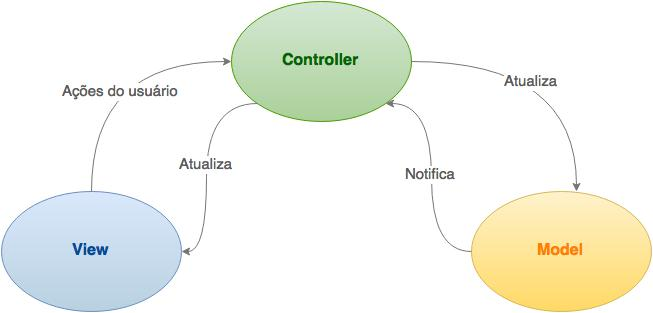
\includegraphics[width=10cm,keepaspectratio]{figuras/MVC.jpg}
\caption{\label{fig:mvc} Arquitetura MVC}
\end{figure}

\textbf{Model:} A camada Model representa a primeira camada de interação com qualquer banco de dados que possa estar sendo usado na aplicação. Ela é responsável por obter, processar, validar dados do banco de dados.

\textbf{View:} A view é responsável por usar as informações disponibilizadas para produzir qualquer interface de apresentação que a aplicação pode necessitar.

\textbf{Controller:} essa camada lida com as requisições dos usuários. É responsável por se comunicar com a camada Model para realizar operações de busca ou armazenamento de dados e repassar os dados obtidos para a camada View, que irá gerar uma saída resultante para o usuário.

MVC é um padrão de projeto de software recomendado para aplicações de desenvolvimento rápido, de fácil manutenção e modular. E foi escolhido como o ideal para um projeto com um tempo limitado de desenvolvimento e possibilita a divisão fácil de tarefas entre os membros da equipe

\section{Wireless Sensor Network }
\label{Sec:WSN}
Wireless Sensor Network, também conhecido como WSN, é um termo genérico que descreve sistemas que tem como objetivo o sensoriamento e monitoração de algum objeto em uma certa área, em pelo menos uma variável (temperatura, umidade, pressão, cor, etc). Os desafios de tais estruturas se resumem a \cite{WSN_survey_JYBMDG_article}: sensores e nós que compõem a rede e podem ter a função de sensoriamento ou de retransmitir dados a um outro nó ou à estação base para serem salvos e devem formar sozinhos uma rede que consiga garantir que os dados sensoriados chegem à base, protocolo de comunicação entre nós, que podem afetar significantemente no consumo de energia, atrasos de comunicação e eficiência do sistema como um todo, fontes de energia dos nós limitada e soluções de coleta de energia. 

\section{Padrão ZigBee e o XBee}
\label{Sec:ZigBee_XBee}
 Para realizar a comunicação sem fio entre os módulos coordenador e sensor, foi necessária a escolha de um padrão para fazer esse intermédio de mensagens. Para realizar tal escolha foram levados em consideração principalmente a eficiência energética que o padrão tem, confiabilidade e escalabilidade. Apesar de existirem opções melhores em certos aspectos, como o Bluetooth Low Energy na área de consumo de energia \cite{BLE_MHABAL}, o ZigBee possui um certo balanceamento das características procuradas, sendo uma solução mais genérica \cite{CG_JP_survey}. Com a existência do XBee, um dispositivo que implementa o ZigBee, é mais interessante adotar tal padrão, uma vez que esse dispositivo facilita a produção do protótipo final.

 O padrão ZigBee e o dispositivo XBee possuem muitas características configuráveis e que podem servir a várias aplicações\cite{xbee_book}, porém duas delas são de maior interesse para o trabalho: o baixo consumo de energia e os modos de operação. O XBee pode ser configurado para operar em um dos dois modos: AT ou API. No modo AT há apenas o envio de dados ponto-a-ponto na rede, porém, no modo API, é possível agir na rede durante sua operação com mudanças de configuração de nós, broadcast, confirmação de entrega de pacotes e identificação do endereço dos dados recebidos, o que dá ao sistema um maior controle do todo \cite{xbee_documentation}
 
\section{Topologias de Rede}
\label{Sec:Redes_topologias}
 Como os nós dos sensores formam uma rede, é necessário analisar as possibilidades de redes.  Como são usados XBees para formar essa rede de sensores, deve-se atentar aos tipos de rede possíveis \cite{xbee_book} \cite{xbee_documentation}.
 
\begin{figure}[H]
\centering
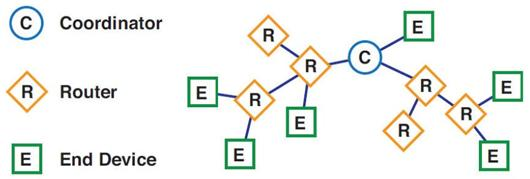
\includegraphics[width=10cm,keepaspectratio]{figuras/zigbee_network_topology.jpg}
\caption{\label{fig:zigbee_network} Topologia de uma rede zigbee}
fonte: \url{http://ftp1.digi.com/support/documentation/html/90001399/90001399_A/Files/XBee-concepts.html}
\end{figure}
 
 A rede ZigBee é composta por nós que podem ser de três tipos:
 \begin{itemize}
\item{Coordenador}: Nó destino (final) de todos os outros nós, concentrando os dados de todos os nós. Todas as redes possuem apenas um nó desse tipo e como esse tipo de nó não possui a capacidade de dormir ele não deveria ficar em um dispositivo com uma bateria limitada.
\item{Roteador}: Funciona apenas como uma ponte intermediária entre os endpoints e o coordenador, podendo se comunicar com todos os outros tipos de nós, mas também não possuem a capacidade de dormir, logo não podem ser energizados com uma bateria limitada. Normalmente são usados para estender a área de uma rede, aumentando o alcance sensoreada da rede como um todo.
\item{Dispositivos finais}: Nós que são as pontas da rede e que normalmente estão ligados aos sensores. Esses tem a capacidade de dormir e conservar energia enquanto não transmitem e só não conseguem se comunicar com outros nós do mesmo tipo diretamente;

Dadas essas especificações e limitações, as redes formadas por esses componentes podem ser de de três tipos \cite{xbee_book}: estrela, árvore ou mesh. Na estrela os dispositivos finais conversam diretamente com o coordenador, na rede mesh os dispositivos finais estão intermediados por uma malha de roteadores que se organizam para encontrar o melhor caminho de roteadores de um dispositivo final até o coordenador e a árvore é um subcaso da rede mesh onde, devido a bloqueios físicos ou distâncias entre os roteadores, a rede acaba por se tornar uma árvore ou um grafo onde o caminho de um dispositivo final até o coordenador praticamente não possui alternativas.

\end{itemize}


\mychapter{Especificação do Projeto}
\label{Cap:especificacao}

O sistema é composto por duas partes: hardware, ou seja, os componentes como microcontroladores, sensores, entre outros; e software, identificado como o aplicativo de interface entre o usuário e os dados coletados.

O sistema está brevemente descrito através da figura \ref{fig:esqueminha} e a disposição dos componentes através do diagrama de implantação da figura \ref{fig:diagrama_implantacao}:

\begin{figure}
\centering
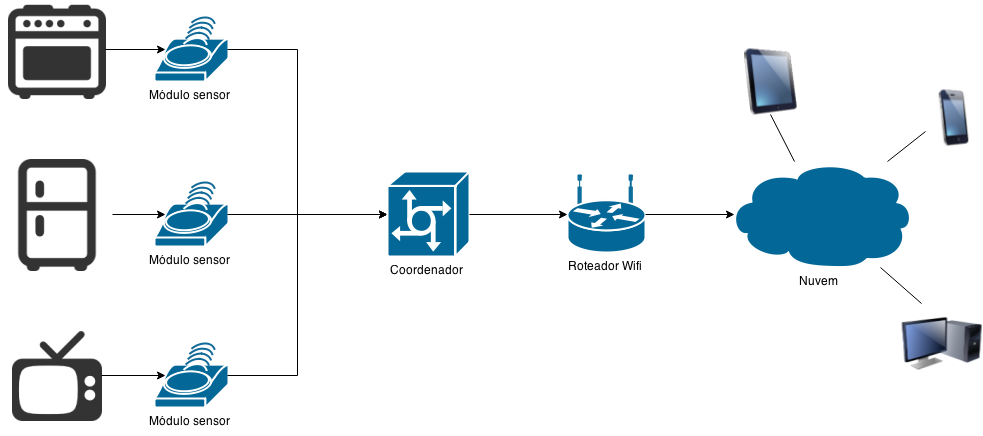
\includegraphics[width=1\textwidth]{figuras/esqueminha.png}
\caption{\label{fig:esqueminha} Esquema do Projeto}
\end{figure}

\begin{figure}
\centering
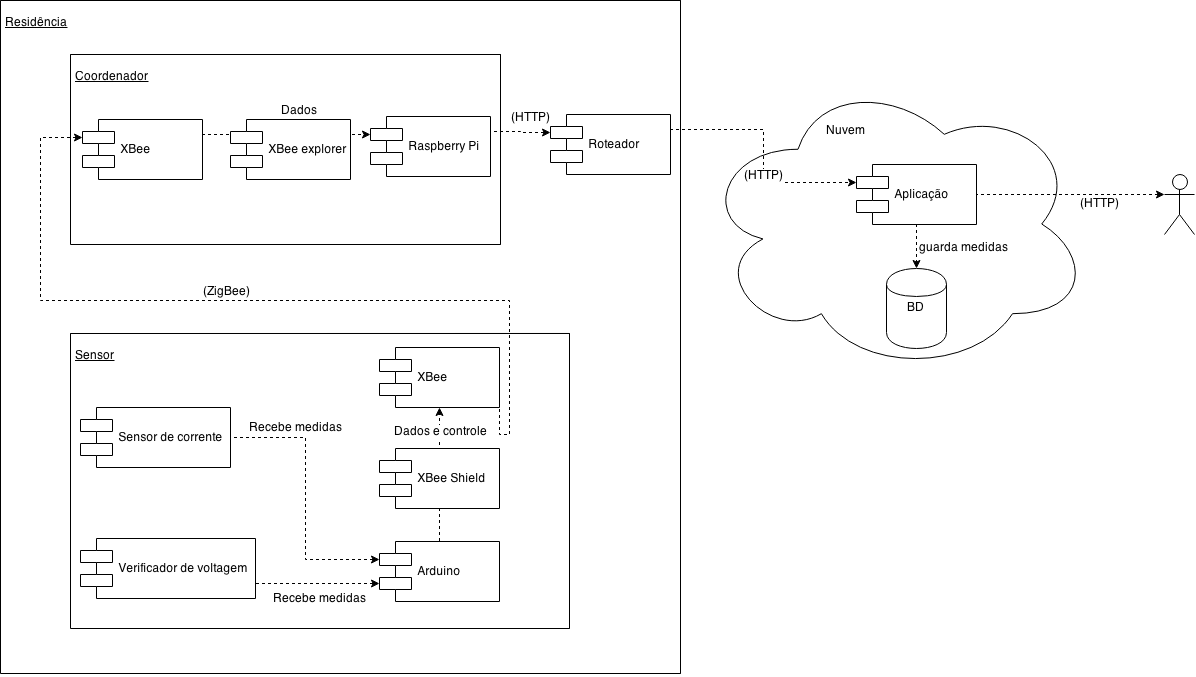
\includegraphics[width=1\textwidth]{figuras/diagrama_implantacao.png}
\caption{\label{fig:diagrama_implantacao} Diagrama de implantação}
\end{figure}

A parte de hardware está separado em dois módulos principais: o módulo de sensoriamento e um módulo coordenador e a parte de software se resume à parte da aplicação web na nuvem.

\section{Escopo}

Coletados os dados, resta mostrar informações úteis ao usuário. Com o consumo de corrente e a voltagem da tomada, é possível calcular a potência e alguns outros dados interessantes para o usuário. O aplicativo desenvolvido nesse trabalho será responsável por esse tratamento e a visualização dos dados coletados pelos sensores. As principais metas são as seguintes:

\begin{itemize}
	\item{informar ao usuário sobre o gasto de energia por equipamento em sua residência}
	\item{auxiliar o usuário a tomar decisões para diminuir o consumo de energia}
  \item{permitir o acesso às informações de consumo tanto localmente quanto remotamente}
\end{itemize}
%
\section{Funções do Sistema}

\begin{description}
	\item[Gerenciar contas:] O usuário poderá fazer cadastro/alteração de conta e autenticação.
	\item[Gerenciar equipamentos:] O usuário poderá fazer criação, edição e remoção de equipamentos, os quais serão monitorados pelo sistema
	\item[Gerenciar sensores:] Os módulos sensores são auto-detectados, e o usuário poderá editar ou removê-los
	\item[Gerenciar metas:] O usuário poderá criar, editar e remover metas mensais.
	\item[Gerenciar consumo:] O módulo coordenador enviará consumos para o sistema estes serão cadastrados. O usuário poderá visualizar os consumos através de gráficos. Além disso o usuário poderá importar ou exportar dados de consumo
	\item[Atualizar taxas da AES:] O usuário poderá atualizar as taxas de energia utilizadas para cálculo do custo do consumo
	\item[Configurar sistema:] O usuário poderá associar os sensores aos equipamentos e escolher um tipo de renda
\end{description}

\section{Requisitos não Funcionais}

\begin{itemize}
	\item{independência do usuário em relação ao técnico do sistema para instalar o sistema em sua residência}
	\item{sistema de fácil manuseio pelo usuário morador da residência}
	\item{os componentes físicos do sistema portáteis}
\end{itemize}

\section{Premissas}

Sendo esse um projeto que visa o sensoriamento e de um monitor para vizualisar os dados com o objetivo de dar uma visão geral ao usuário sobre gastos supérfulos e uma relação absoluta do consumo de cada equipamento, o sistema é influenciado por alguns fatores físicos e geopolíticos, o que leva à necessidade de usar algumas premissas que tiveram de ser feitas para ajustar o projeto ao tempo previsto e garantir o funcionamento correto do sistema:

\begin{enumerate}
\item{O usuário deve morar em São Paulo}
\item{Será considerado um fator de potência ideal unitário}
\end{enumerate}
\section{Hardware}
\label{Sec:hardware}
\subsection{Módulo sensor}

O módulo sensor vai ser responsável por medir e transmitir as informações necessárias para calcular o consumo de energia do equipamento acoplado.

Os componentes físicos do módulo sensor são:

\begin{itemize}
\item Circuito Verificador de tensão
\item Sensor de Corrente (Non-invasive AC Current Sensor)
\item Arduino Uno - R3
\item XBee Shield
\item XBee 2mW PCB Antenna - Series 2
\end{itemize}
%
\subsection{Coordenador}

O módulo coordenador vai ser responsável por fazer requisições para os módulos sensores, tratar os dados de consumo e enviar ao aplicativo na nuvem.

Os componentes do coordenador são:

\begin{itemize}
\item Kit Raspberry Pi2 + Fonte + Microsd 8gb + Wifi Usb
\item XBee Explorer Dongle
\item XBee 2mW PCB Antenna - Series 2
\end{itemize}
%
\subsection{Circuitos}
\subsubsection{Verificador de Tensão}

No circuito de cada módulo de sensor, são feitas detecções da tensão (127V ou 220V) para cálculos de potência.  O objetivo do circuito da figura \ref{fig:voltage-circuit} é indicar se a tensão na tomada é 220V ou 127V. A saída do circuito é usada como um valor analógico, que dependendo da tensão de entrada resultará em faixas diferentes para as diferentes tensões.

\begin{figure}[H]
\centering
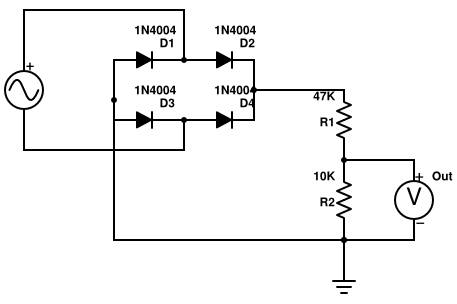
\includegraphics[width=9cm,keepaspectratio]{figuras/voltage-circuit.jpg}
\caption{\label{fig:voltage-circuit} Circuito verificador de tensão}
\end{figure}

\subsubsection{Medidor de Corrente}

Ainda no módulo sensor, é necessário obter as medidas do valor eficaz da corrente. O sensor não-invasivo produz uma tensão alternada na saída, e antes da coleta de dados pelo arduino é preciso obter um valor significativo, que não ultrapasse 2.5V. Para isso foi utilizado o circuito da figura \ref{fig:sensor-circuit}.

\begin{figure}[H]
\centering
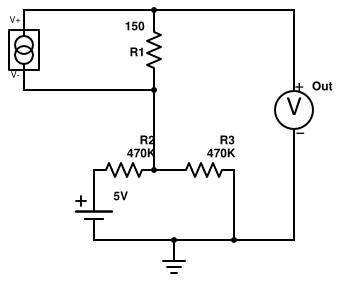
\includegraphics[width=9cm,keepaspectratio]{figuras/current-circuit.jpg}
\caption{\label{fig:sensor-circuit} Circuito medidor de corrente}
\end{figure}
%
\subsection{Peças}
\subsubsection{Sensor de Corrente Não-invasivo AC}
\begin{figure}[H]
\begin{center}
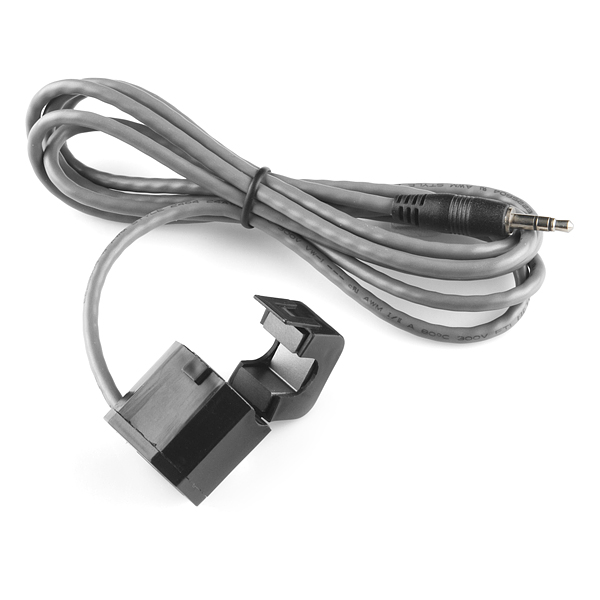
\includegraphics[width=5cm,height=5cm,keepaspectratio]{figuras/sensor.jpg}
\caption{\label{fig:sensor} Non-invasive AC current sensor}
\end{center}
\end{figure}

Esse sensor de corrente consegue medir a corrente que passa por um fio de modo não-invasivo. O sensor funciona como um transformador respondendo a um campo magnético formado em volta do fio condutor. Este, em particular, suporta até 30A de entrada, e necessita de um resistor de saída para obter a medida desejada em tensão.

\begin{itemize}
\item{Corrente suportada: 30A}
\item{Temperatura de operação: -40$^{\circ}$C até 65 $^{\circ}$C}
\item{Precisão de 2\%}
\end{itemize}
%
\subsubsection{Raspberry Pi 2 modelo B}
\begin{figure}[H]
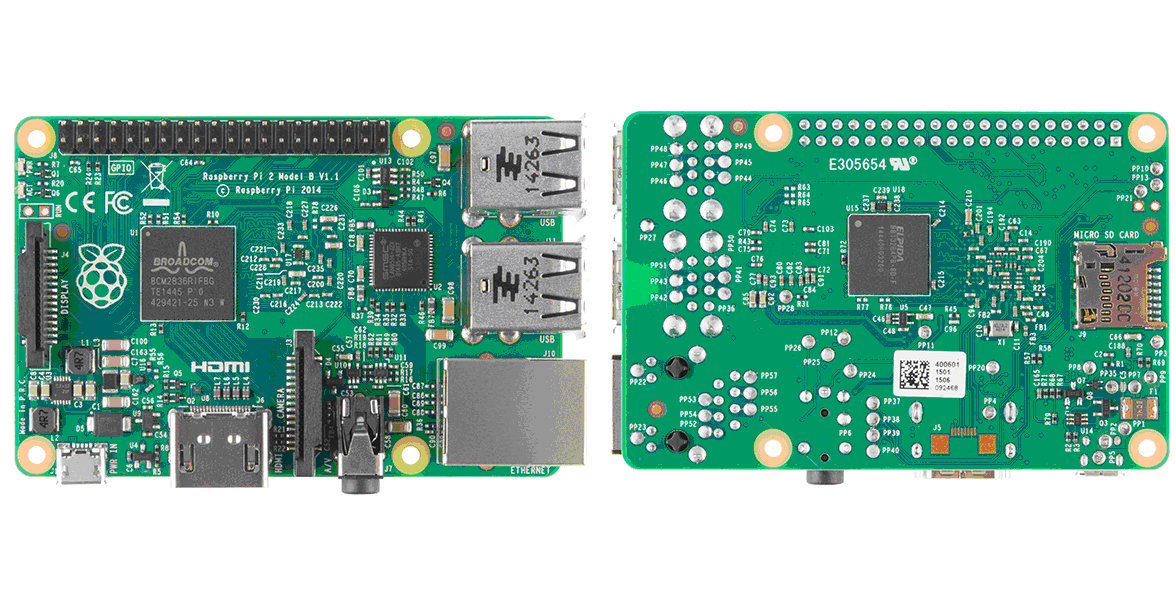
\includegraphics[width=1\textwidth]{figuras/raspberry_pi.png}
\caption{\label{fig:raspberry pi} Raspberry pi 2 modelo B}
\end{figure}

A Raspberry Pi 2 Modelo B (figura \ref{fig:raspberry pi}) é o computador utilizado no sistema para receber os dados enviados pelos módulos sensores, tratá-los e enviar para o aplicativo. Foi escolhido o Raspberry Pi 2 - Model B por ser mais veloz, por possuir mais entradas USB e ser de alta disponibilidade no mercado, por um preço razoável. O kit inclui a fonte, um cartão microSD de 8GB e um adaptador Wifi USB.

\begin{itemize}
\item{A 900MHz quad-core ARM Cortex-A7 CPU}
\item{1GB RAM}
\item{40 pinos GPIO}
\item{saída Full HDMI}
\item{porta Ethernet}
\item{entrada para cartão Micro SD}
\item{4 entradas USB}
\end{itemize}
%
\subsubsection{Arduino UNO}
\begin{figure}[H]
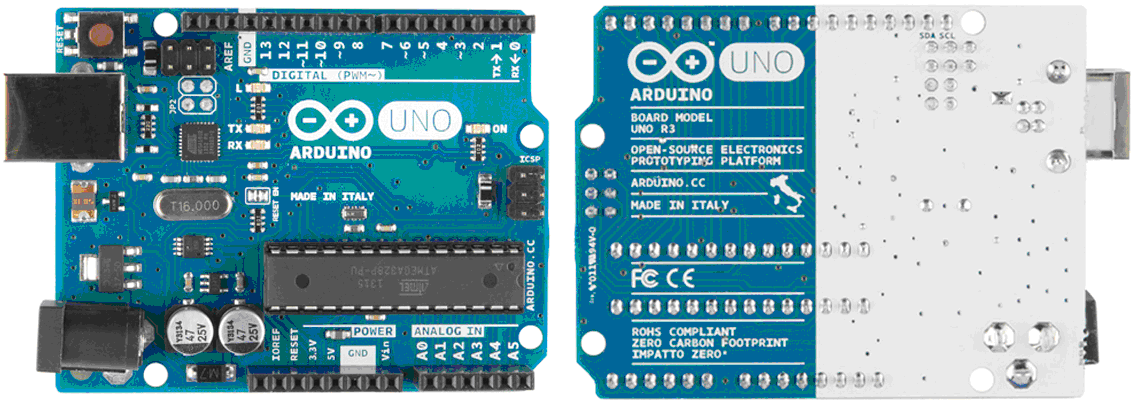
\includegraphics[width=1\textwidth]{figuras/arduino_uno.png}
\caption{\label{fig:arduino uno} Arduino UNO R3}
\end{figure}

Arduino é uma placa programável open-source . No projeto em questão esse componente receberá os dados do sensor, fará um tratamento e terá o envio programado desses para o coordenador. Pelo Arduino ser programável e possuir uma interface muito amigável, simplifica essa ponte entre a coleta de dados e a transmissão. E sua alta disponibilidade no mercado , assim como o raspberry, facilita sua obtenção.

\begin{itemize}
\item{microcontrolador ATmega328}
\item{tensão de entrada - 7-12V}
\item{14 Pinos Digital I/O (6 PWM de saída)}
\item{6 Inputs Analógicos}
\item{32k de memória Flash}
\item{16Mhz de Relógio}
\end{itemize}
%
\subsubsection{XBee}
\begin{figure}[H]
\begin{center}
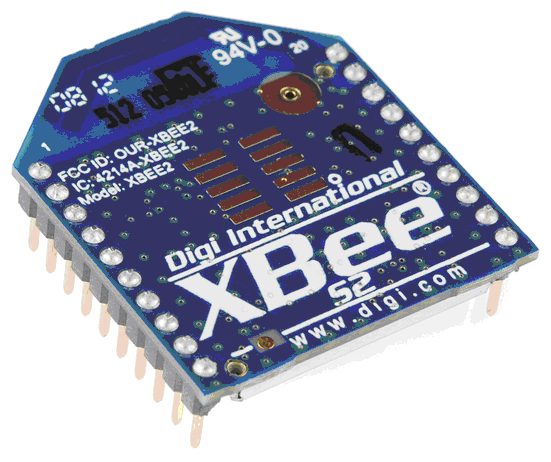
\includegraphics[width=5cm,height=5cm,keepaspectratio]{figuras/xbee_serie2.png}
\caption{\label{fig:xbee} XBee Serie 2}
\end{center}
\end{figure}

É um módulo que permite uma comunicação simples e confiável entre microcontroladores, computadores, sistemas através de uma porta serial com um consumo menor de energia. Pode ser utilizado em redes ponto-a-ponto e multi-ponto. Foram escolhidos módulos da série 2 por serem configuráveis.
Algumas outras especificações são:

\begin{itemize}
\item{entradas de 3.3V @ 40mA}
\item{transmissão de dados máxima de 250kbps}
\item{potência de saída: 2mW (+3dBm)}
\item{alcance máximo de 120m}
\item{08 pinos digitais entrada/saída}
\item{encriptação 128-bit}
\item{configuração local ou remota}
\item{conector de antena RPSMA}
\end{itemize}
%
\subsubsection{XBee Explorer Dongle}
\begin{figure}[H]
\begin{center}
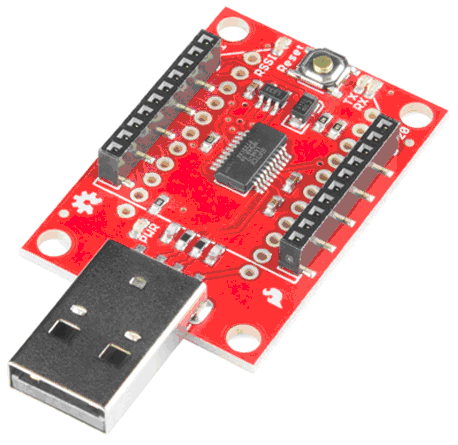
\includegraphics[width=5cm,height=5cm,keepaspectratio]{figuras/xbee_explorer_dongle.png}
\caption{\label{fig:xbee explorer dongle} XBee Explorer Dongle}
\end{center}
\end{figure}

É um módulo com porta USB que faz a conexão do módulo XBee a um computador. Isso é necessário para ter acesso aos pinos de comunicação serial e de programação. Ele possui um conversor serial, que traduz os dados entre o computador e o XBee. Possui um botão de reset e um regulador de tensão para suprir a tensão necessária para XBee. Além disso possui 4 leds para debug: RX, TX, RSSI e indicador de energia. No projeto, este módulo é utilizado para fazer as configurações iniciais de todos os XBees e para conectar o XBee coordenador ao Raspberry Pi. Apesar de não ser um dispositivo essencial, este facilita muito nas tarefas citadas,  principalmente por lidar com a alimentação de 3,3V do XBee.

\subsubsection{XBee Shield}
\begin{figure}[H]
\begin{center}
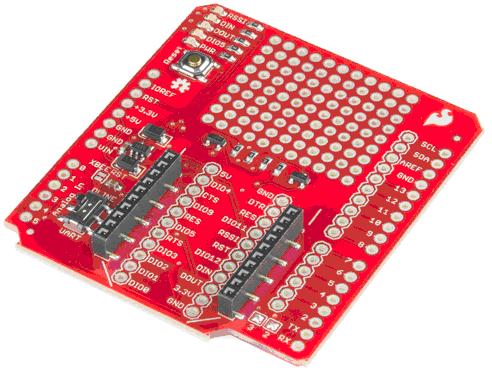
\includegraphics[width=5cm,height=5cm,keepaspectratio]{figuras/xbee_shield.png}
\caption{\label{fig:xbee shield} XBee shield do arduino UNO}
\end{center}
\end{figure}

É um módulo que faz a conexão entre um módulo XBee e um Arduino. Ele possui opções para escolher se a conexão vai ser nos pinos UART ou qualquer outros pinos digitais do Arduino. A alimentação de 5V vinda do Arduino é regulada para 3.3V VDC antes de chegar no módulo XBee. O XBee Shield inclui LEDs para indicar a utilização dos pinos DIN, DOUT, RSSI e DIO5 do XBee. É usado um módulo XBee Shield para cada par XBee + Arduino.

\subsubsection{Arduino Stackable Header Kit - R3}
\begin{figure}[H]
\begin{center}
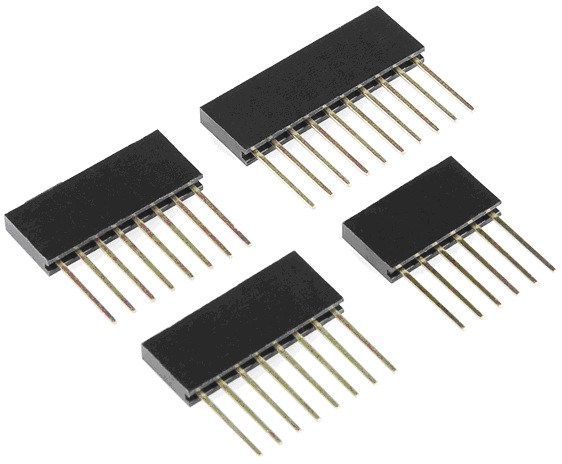
\includegraphics[width=5cm,height=5cm,keepaspectratio]{figuras/headers.png}
\caption{\label{fig:xbee shield headers} Headers usados no XBee shield}
\end{center}
\end{figure}

São conectores usados para encaixar o módulo XBee Shield no Arduino Uno R3. Estão inclusos 4 headers, 2 x 8 pinos, 1 x 10 pinos e 1 x 6 pinos, suficientes para 1 módulo XBee Shield. Como há 2 sensores no projeto, serão usados 2 kits, com um adicional de reserva.



\section{Software}
\label{Sec:software}

\subsection{Classes e atributos}

A seguir estão descritas as classes do sistema e seus respectivos atributos. As classes implementadas estão representadas pelo diagrama de classes (figura \ref{fig:diagrama-classes}).

\begin{figure}[H]
\begin{center}
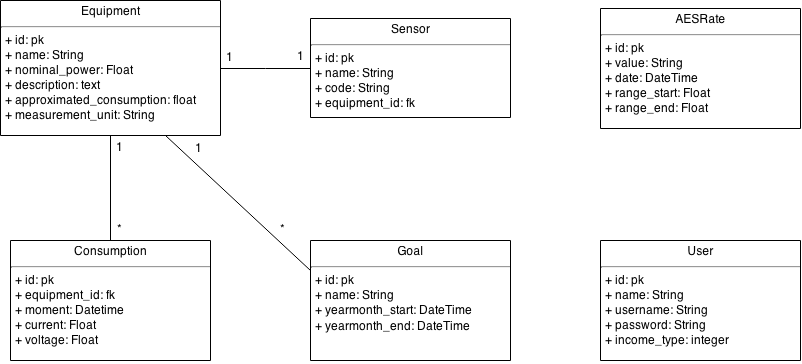
\includegraphics[width=10cm,height=10cm,keepaspectratio]{figuras/diagrama_classes.png}
\caption{\label{fig:diagrama-classes} Diagrama de Classes}
\end{center}
\end{figure}

\subsubsection{Equipment}
\begin{description}
	\item[Classe:] Equipment
	\item[Descrição:] um equipamento monitorado
	\item[Atributos:]
\end{description} 
\begin{enumerate}
  \item id (integer): Identificador do equipamento
  \item name (String): Nome do equipamento
  \item description (Text): descrição do equipamento 
  \item nominal\_power (float): potência do equipamento descrita no manual do equipamento 
  \item measurement\_unit (String): unidade do valor dado em nominal\_power
  \item approximated\_consumption (float): consumo aproximado do equipamento dado pelo fabricante 
\end{enumerate}
%
\subsubsection{Sensor}
\begin{description}
	\item[Classe:] Sensor
	\item[Descrição:] um sensor do sistema
	\item[Atributos:]
\end{description} 
\begin{enumerate}
	\item id (integer): identificador do sensor dentro do software.
	\item name (String): nome dado pelo usuário para o sensor
	\item code (String): identificador do sensor entre outros sensores. Informação configurada no próprio módulo do sensor.
	\item equipment\_id (integer): equipamento a qual está associado
\end{enumerate}
%
\subsubsection{Consumption}
\begin{description}
	\item[Classe:] Consumption
	\item[Descrição:] Representa uma medida feita de um equipamento em um dado instante
	\item[Atributos:]
\end{description} 
\begin{enumerate}
	\item id (integer): identificador do consumo
	\item moment (DateTime): a data e a hora de quando foi feita a medida
	\item current (float): corrente no momento da medida em amperes
	\item voltage (float): voltagem do tomada do equipamento. 220V ou 110V
\end{enumerate}
%
\subsubsection{User}
\begin{description}
	\item[Classe:] User
	\item[Descrição:] Representa um usuário do sistema
	\item[Atributos:]
\end{description} 
\begin{enumerate}
	\item id (integer): identificador do usuário
	\item name (String):  Nome do usuário
	\item username (String): Nome de usuário usado para efetuar o login
	\item password (String com Criptografia): Senha do usuário usada para efetuar o login
    \item income\_type (String): O tipo de renda do usuário, Residencial ou Residencial de baixa renda, definida pela AES eletropaulo.
\end{enumerate}
%
\subsubsection{Goal}
\begin{description}
	\item[Classe:] Goal
	\item[Descrição:] Representa uma meta de consumo por mês
	\item[Atributos:]
\end{description} 
\begin{enumerate}
	\item id (integer): identificador da meta
	\item name (String):  Nome da meta
	\item value\_in\_percent (float): Consumo pretendido em percentagem (em relação ao mês anterior)
	\item yearmonth\_start (DateTime): Mês/Ano de início do período da meta
    \item yearmonth\_end (DateTime): Mês/Ano de fim do período da meta
\end{enumerate}
%
\subsubsection{AESRate}
\begin{description}
	\item[Classe:] AESRate
	\item[Descrição:] Representa a taxa de conversão da AES eletropaulo de kilowatts hora para reais. Esses valores obtidos através da página de tarifas do site da AES Eletropaulo \cite{aes_site}
	\item[Atributos:]
\end{description} 
\begin{enumerate}
	\item id (integer): identificador da taxa de conversão
	\item value (float): O valor da taxa de conversão no instante
	\item date (DateTime): O instante que a taxa de conversão foi buscada
	\item range\_start (float): O início da faixa que define a taxa de conversão
    \item range\_end (float): O início da faixa que define a taxa de conversão
\end{enumerate}

No sistema é possível cadastrar apenas uma entidade principal os equipamentos eletrônicos monitorados, sendo prevista a possibilidade de que um sensor possa mudar de um equipamento para outro, sendo que tal mudança deve ser cadastrada no sistema pelo  usuário na tela de configurações, como mostrado na tela de configurações no diagrama de navegação (figura \ref{fig:diagrama-navegacao}).  Essa possibilidade de mudança da configuração dos sensores explica a relação do equipamento e as medidas de consumo: caso o usuário troque o sensor de equipamento ainda será possível visualizar dados anteriores de outros equipamentos já monitorados.

Os sensores devem ser criados automaticamente pelo sistema uma vez que eles sejam colocados no sistema. Eles enviam um sinal inicial que informa seu identificador para que o sistema o cadastre. O usuário poderá, então, colocar um nome que preferir nesse sensor. Porém, como não há qualquer informação que o sistema pode indicar ao sistema em qual aparelho ou em que tipo de aparelho o sensor foi instalado, tal associação deve ser feita manualmente antes que os dados comecem a ser coletados.

Adquiridas as medidas, é possível vizualizar esses dados em uma tabela de consumo na tela de consumo. Nessa tela, é possível construir o gráfico do consumo em função de vários períodos de tempo, no caso, o consumo por dia e por mês, assim como metas de consumo de energia dos equipamentos selecionados e previsões de consumo que serão calculadas a partir do consumo nominal dos equipamentos.

\begin{figure}[H]
\begin{center}
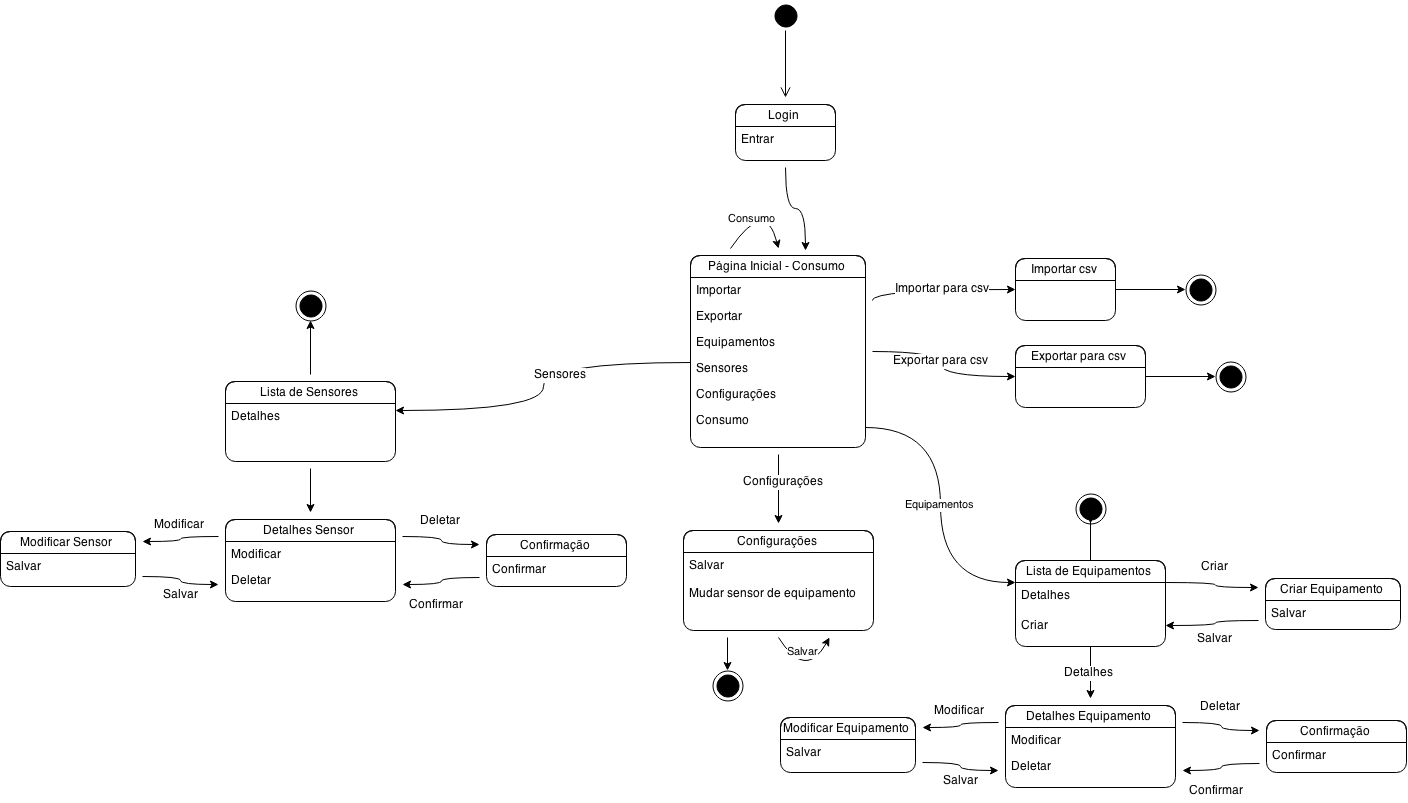
\includegraphics[width=10cm,height=10cm,keepaspectratio]{figuras/diagrama_navegacao.png}
\caption{\label{fig:diagrama-navegacao} Diagrama de Navegação}
\end{center}
\end{figure}
%
\subsection{Atores}
\begin{description}
	\item[usuário:] Como o sistema vai ser utilizado apenas pelo(s) responsável(is) pela residência, há apenas um tipo de usuário, que é o usuário comum
    \item[módulo coordenador:] É o componente de hardware que enviará informações de consumo para o sistema
\end{description}
\subsection{Casos de uso}

Os casos de uso do sistema estão listados na tabela \ref{tab:casos_de_uso}.

\begin{table}
\centering
{\renewcommand{\arraystretch}{1.5}
\renewcommand{\tabcolsep}{0.2cm}
\begin{tabular}{|c|c|}
\hline
\textbf{Funções} & \textbf{Casos de uso} \\
\hline
\multirow{4}{*}{Gerenciar conta} & Fazer cadastro\\
& Fazer login\\
& Fazer logout\\
& Recuperar senha\\
\hline
\multirow{3}{*}{Gerenciar equipamentos} & Criar equipamento\\
& Editar equipamento\\
& Remover equipamento\\
\hline
\multirow{3}{*}{Gerenciar sensores} & Detectar sensores\\
& Editar sensor\\
& Remover sensor\\
\hline
\multirow{3}{*}{Gerenciar metas} & Criar meta\\
& Editar meta\\
& Remover meta\\
\hline
\multirow{4}{*}{Gerenciar consumo} & Criar consumo\\
& Visualizar consumo\\
& Importar consumo\\
& Exportar consumo\\
\hline
Atualizar taxas da AES & Atualizar taxas da AES\\
\hline
Configurar sistema & Configurar sistema\\
\hline
\end{tabular}}
\caption{\label{tab:casos_de_uso} Casos de Uso.}
\end{table}
%
\subsection{Descrição dos casos de uso}

A seguir são descritos os casos de uso do sistema. 

% ************************************************
% 1 - GERENCIAR CONTA
% ************************************************
\subsubsection{Caso de Uso 1: Gerenciar conta}
\subsubsection{Caso de Uso 1.1: Fazer cadastro}
\begin{description}
	\item[Descrição:] inserção de um novo usuário comum no sistema
	\item[Evento iniciador:] solicitação de cadastro
	\item[Atores:] usuário
	\item[Pré-condição:] sistema exibindo tela de solicitação de cadastro
	\item[Sequência de eventos:] \hfill
		\begin{enumerate}
			\item{Usuário solicita cadastro}
			\item{Sistema exibe o formulário de cadastro}
			\item{Usuário insere os seus dados}
			\item{Sistema insere o novo usuário e exibe o resultado}
		\end{enumerate}
	\item[Pós-condição:] novo usuário cadastrado, usuário é logado automaticamente e é exibida a tela inicial
	\item[Extensões:] \hfill
		\begin{enumerate}
			\item{\textbf{Usuário a ser cadastrado já existe:} sistema apresenta uma mensagem ao usuário (passo 4)}
			\item{\textbf{Dados do usuário não consistentes:} sistema apresenta mensagem de erro ao usuário (passo 4)}
		\end{enumerate}
	\item[Inclusões:] \hfill
		\begin{enumerate}
			\item{Buscar usuário (passo 4)}
		\end{enumerate}
\end{description}
%
\subsubsection{Caso de Uso 1.2: Fazer login}
\begin{description}
	\item[Descrição:] criar uma sessão do usuário no sistema
	\item[Evento iniciador:] solicitação de login
	\item[Atores:] usuário
	\item[Pré-condição:] usuário cadastrado e não há usuário logado
	\item[Sequência de eventos:] \hfill
		\begin{enumerate}
			\item{usuário solicita login}
			\item{sistema exibe formulário para login}
			\item{usuário insere os dados de login}
			\item{sistema cria uma sessão para o usuário e redireciona para a página inicial}
		\end{enumerate}
	\item[Pós-condição:] sessão criada e sistema exibe a tela inicial
	\item[Extensões:] \hfill
		\begin{enumerate}
			\item{\textbf{Usuário não encontrado:} sistema apresenta uma mensagem de erro ao usuário (passo 4)}
			\item{\textbf{Dados não consistentes:} sistema apresenta uma mensagem de erro ao usuário (passo 4)}
		\end{enumerate}
	\item[Inclusões:] \hfill
		\begin{enumerate}
			\item{Buscar usuário (passo 4)}
		\end{enumerate}
\end{description}
%
\subsubsection{Caso de Uso 1.3: Fazer logout}
\begin{description}
	\item[Descrição:] encerrar a sessão do usuário atual no sistema
	\item[Evento iniciador:] solicitação de logout
	\item[Atores:] usuário
	\item[Pré-condição:] usuário logado
	\item[Sequência de eventos:] \hfill
		\begin{enumerate}
			\item{usuário solicita logout}
			\item{sistema encerra a sessão atual, e redireciona para a página de login}
		\end{enumerate}
	\item[Pós-condição:] sessão encerrada e sistema exibe tela de login
\end{description}
%
\subsubsection{Caso de Uso 1.4: Recuperar senha}
\begin{description}
	\item[Descrição:] recuperar a senha do usuário
	\item[Evento iniciador:] solicitação de recuperação de senha
	\item[Atores:] usuário
	\item[Pré-condição:] usuário cadastrado, não há usuário logado e sistema exibindo tela de login
	\item[Sequência de eventos:] \hfill
		\begin{enumerate}
			\item{usuário solicita recuperação de senha}
			\item{sistema exibe formulário para recuperação de senha}
			\item{usuário insere o e-mail}
			\item{sistema envia e-mail para recuperar a senha e exibe mensagem}
			\item{usuário clica no link para recuperar senha no e-mail}
			\item{sistema exibe o formulário para recuperar a senha}
			\item{usuário insere os dados pedidos}
			\item{sistema atualiza a senha do usuário, autentica o usuário e redireciona para a tela inicial}
		\end{enumerate}
	\item[Pós-condição:] senha do usuário atualizada, usuário autenticado e sistema mostra a tela inicial
	\item[Extensões:] \hfill
		\begin{enumerate}
			\item{\textbf{Dados não consistentes:} sistema apresenta uma mensagem de erro ao usuário (passo 4, 8)}
			\item{\textbf{Senha antiga incorreta:} sistema apresenta uma mensagem de erro ao usuário (passo 8)}
		\end{enumerate}
	\item[Inclusões:] \hfill
		\begin{enumerate}
			\item{Buscar usuário (passo 8)}
		\end{enumerate}
\end{description}
% ************************************************
% 2 - GERENCIAR EQUIPAMENTO
% ************************************************
\subsubsection{Caso de Uso 2: Gerenciar equipamentos}
\subsubsection{Caso de Uso 2.1: Criar equipamento}
\begin{description}
	\item[Descrição:] criar um novo equipamento
	\item[Evento iniciador:] solicitação de criação de equipamento
	\item[Atores:] usuário
	\item[Pré-condição:] usuário logado e sistema exibindo listagem de equipamentos
	\item[Sequência de eventos:] \hfill
		\begin{enumerate}
			\item{usuário solicita criação de equipamento}
			\item{sistema exibe formulário para criação}
			\item{usuário insere os dados para criação}
			\item{sistema cria um equipamento e redireciona para a listagem de equipamentos}
		\end{enumerate}
	\item[Pós-condição:] equipamento criado e sistema exibe listagem de equipamentos
	\item[Extensões:] \hfill
		\begin{enumerate}
			\item{\textbf{Dados não consistentes:} sistema apresenta uma mensagem de erro ao usuário (passo 4)}
			\item{\textbf{Equipamento já existe:} sistema apresenta uma mensagem de erro ao usuário (passo 4)}
		\end{enumerate}
	\item[Inclusões:] \hfill
		\begin{enumerate}
			\item{Buscar equipamento (passo 4)}
		\end{enumerate}
\end{description}
%
\subsubsection{Caso de Uso 2.2: Editar equipamento}
\begin{description}
	\item[Descrição:] editar um equipamento
	\item[Evento iniciador:] solicitação de edição de equipamento
	\item[Atores:] usuário
	\item[Pré-condição:] usuário logado, existem equipamentos e sistema exibindo listagem de equipamentos
	\item[Sequência de eventos:] \hfill
		\begin{enumerate}
			\item{usuário seleciona o equipamento desejado para edição}
			\item{sistema exibe formulário para edição}
			\item{usuário altera os dados desejados}
			\item{sistema atualiza o equipamento e redireciona para a listagem de equipamentos}
		\end{enumerate}
	\item[Pós-condição:] equipamento atualizado e sistema exibe listagem de equipamentos
	\item[Extensões:] \hfill
		\begin{enumerate}
			\item{\textbf{Dados não consistentes:} sistema apresenta uma mensagem de erro ao usuário (passo 4)}
		\end{enumerate}
	\item[Inclusões:] \hfill
		\begin{enumerate}
			\item{Buscar equipamento (passo 2, 4)}
		\end{enumerate}
\end{description}
%
\subsubsection{Caso de Uso 2.3: Remover equipamento}
\begin{description}
	\item[Descrição:] remover um equipamento
	\item[Evento iniciador:] solicitação de remoção de equipamento
	\item[Atores:] usuário
	\item[Pré-condição:] usuário logado, existem equipamentos e sistema exibindo listagem de equipamentos
	\item[Sequência de eventos:] \hfill
		\begin{enumerate}
			\item{usuário seleciona o equipamento desejado para remoção}
			\item{sistema pede confirmação para remoção}
			\item{usuário confirma}
			\item{sistema remove o equipamento e redireciona para a listagem de equipamentos}
		\end{enumerate}
	\item[Pós-condição:] equipamento removido e sistema exibe listagem de equipamentos
	\item[Extensões:] \hfill
		\begin{enumerate}
			\item{\textbf{Usuário não confirma:} sistema não remove e volta para a tela de listagem (passo 4)}
		\end{enumerate}
	\item[Inclusões:] \hfill
		\begin{enumerate}
			\item{Buscar equipamento (passo 2, 4)}
		\end{enumerate}
\end{description}
% ************************************************
% 3 - GERENCIAR SENSORES
% ************************************************
\subsubsection{Caso de Uso 3: Gerenciar sensores}
\subsubsection{Caso de Uso 3.1: Detectar sensor}
\begin{description}
	\item[Descrição:] detectar um sensor
	\item[Evento iniciador:] solicitação de detecção de sensores
	\item[Atores:] usuário
	\item[Pré-condição:] usuário logado e sistema exibindo listagem de sensores
	\item[Sequência de eventos:] \hfill
		\begin{enumerate}
			\item{usuário solicita detecção de sensor}
			\item{sistema detecta e cria um sensor no sistema com status ativo e atualiza a lista de sensores}
		\end{enumerate}
	\item[Pós-condição:] sensor criado e sistema exibe listagem de sensores
	\item[Extensões:] \hfill
		\begin{enumerate}
			\item{\textbf{Sensor já existe no sistema:} sistema atualiza o status do sensor para ativo (passo 2)}
		\end{enumerate}
	\item[Inclusões:] \hfill
		\begin{enumerate}
			\item{Buscar sensor (passo 2)}
		\end{enumerate}
\end{description}
%
\subsubsection{Caso de Uso 3.2: Editar sensor}
\begin{description}
	\item[Descrição:] editar um sensor
	\item[Evento iniciador:] solicitação de edição de sensor
	\item[Atores:] usuário
	\item[Pré-condição:] usuário logado, existem sensores e sistema exibindo listagem de sensores
	\item[Sequência de eventos:] \hfill
		\begin{enumerate}
			\item{usuário seleciona o sensor desejado para edição}
			\item{sistema exibe formulário para edição}
			\item{usuário altera os dados desejados}
			\item{sistema atualiza o sensor e redireciona para a listagem de sensores}
		\end{enumerate}
	\item[Pós-condição:] sensor atualizado e sistema exibe listagem de sensores
	\item[Extensões:] \hfill
		\begin{enumerate}
			\item{\textbf{Dados não consistentes:} sistema apresenta uma mensagem de erro ao usuário (passo 4)}
		\end{enumerate}
	\item[Inclusões:] \hfill
		\begin{enumerate}
			\item{Buscar sensor (passo 2, 4)}
		\end{enumerate}
\end{description}
%
\subsubsection{Caso de Uso 3.3: Remover sensor}
\begin{description}
	\item[Descrição:] remover um sensor
	\item[Evento iniciador:] solicitação de remoção de sensor
	\item[Atores:] usuário
	\item[Pré-condição:] usuário logado, existem sensores e sistema exibindo listagem de sensores
	\item[Sequência de eventos:] \hfill
		\begin{enumerate}
			\item{usuário seleciona o sensor desejado para remoção}
			\item{sistema pede confirmação para remoção}
			\item{usuário confirma}
			\item{sistema remove o sensor e redireciona para a listagem de sensores}
		\end{enumerate}
	\item[Pós-condição:] sensor removido e sistema exibe listagem de sensores
	\item[Extensões:] \hfill
		\begin{enumerate}
			\item{\textbf{Usuário não confirma:} sistema não remove e volta para a tela de listagem (passo 4)}
		\end{enumerate}
	\item[Inclusões:] \hfill
		\begin{enumerate}
			\item{Buscar sensor (passo 2, 4)}
		\end{enumerate}
\end{description}
% ************************************************
% 4 - GERENCIAR META
% ************************************************
\subsubsection{Caso de Uso 4: Gerenciar metas}
\subsubsection{Caso de Uso 4.1: Criar meta}
\begin{description}
	\item[Descrição:] criar uma nova meta
	\item[Evento iniciador:] solicitação de criação de meta
	\item[Atores:] usuário
	\item[Pré-condição:] usuário logado e sistema exibindo listagem de metas
	\item[Sequência de eventos:] \hfill
		\begin{enumerate}
			\item{usuário solicita criação de meta}
			\item{sistema exibe formulário para criação}
			\item{usuário insere os dados para criação}
			\item{sistema cria uma meta e redireciona para a listagem de metas}
		\end{enumerate}
	\item[Pós-condição:] meta criada e sistema exibe listagem de metas
	\item[Extensões:] \hfill
		\begin{enumerate}
			\item{\textbf{Dados não consistentes:} sistema apresenta uma mensagem de erro ao usuário (passo 4)}
			\item{\textbf{Meta já existe:} sistema apresenta uma mensagem de erro ao usuário (passo 4)}
		\end{enumerate}
	\item[Inclusões:] \hfill
		\begin{enumerate}
			\item{Buscar meta (passo 4)}
		\end{enumerate}
\end{description}
%
\subsubsection{Caso de Uso 4.2: Editar meta}
\begin{description}
	\item[Descrição:] editar uma meta
	\item[Evento iniciador:] solicitação de edição de meta
	\item[Atores:] usuário
	\item[Pré-condição:] usuário logado, existem metas e sistema exibindo listagem de metas
	\item[Sequência de eventos:] \hfill
		\begin{enumerate}
			\item{usuário seleciona a meta desejado para edição}
			\item{sistema exibe formulário para edição}
			\item{usuário altera os dados desejados}
			\item{sistema atualiza a meta e redireciona para a listagem de metas}
		\end{enumerate}
	\item[Pós-condição:] meta atualizada e sistema exibe listagem de metas
	\item[Extensões:] \hfill
		\begin{enumerate}
			\item{\textbf{Dados não consistentes:} sistema apresenta uma mensagem de erro ao usuário (passo 4)}
		\end{enumerate}
	\item[Inclusões:] \hfill
		\begin{enumerate}
			\item{Buscar meta (passo 2, 4)}
		\end{enumerate}
\end{description}
%
\subsubsection{Caso de Uso 4.3: Remover meta}
\begin{description}
	\item[Descrição:] remover uma meta
	\item[Evento iniciador:] solicitação de remoção de meta
	\item[Atores:] usuário
	\item[Pré-condição:] usuário logado, existem metas e sistema exibindo listagem de metas
	\item[Sequência de eventos:] \hfill
		\begin{enumerate}
			\item{usuário seleciona a meta desejado para remoção}
			\item{sistema pede confirmação para remoção}
			\item{usuário confirma}
			\item{sistema remove a meta e redireciona para a listagem de metas}
		\end{enumerate}
	\item[Pós-condição:] meta removida e sistema exibe listagem de metas
	\item[Extensões:] \hfill
		\begin{enumerate}
			\item{\textbf{Usuário não confirma:} sistema não remove e volta para a tela de listagem (passo 4)}
		\end{enumerate}
	\item[Inclusões:] \hfill
		\begin{enumerate}
			\item{Buscar meta (passo 2, 4)}
		\end{enumerate}
\end{description}
% ************************************************
% 5 - GERENCIAR CONSUMO
% ************************************************
\subsubsection{Caso de Uso 5: Gerenciar consumos}
\subsubsection{Caso de Uso 5.1: Criar consumo}
\begin{description}
	\item[Descrição:] inserir consumos no sistema
	\item[Evento iniciador:] solicitação para criação de consumo
	\item[Atores:] módulo coordenador
	\item[Pré-condição:] módulo coordenador ligado e sistema online
	\item[Sequência de eventos:] \hfill
		\begin{enumerate}
			\item{módulo coordenador solicita criação de consumo}
			\item{sistema cria o consumo}
		\end{enumerate}
	\item[Pós-condição:] consumo criado
	\item[Extensões:] \hfill
		\begin{enumerate}
			\item{\textbf{Perda de conexão:} consumo não é criado (passo 2)}
		\end{enumerate}
\end{description}
%
\subsubsection{Caso de Uso 5.2: Visualizar consumo}
\begin{description}
	\item[Descrição:] visualizar os consumos na forma de gráficos
	\item[Evento iniciador:] solicitação de geração de gráfico
	\item[Atores:] usuário
	\item[Pré-condição:] usuário logado, existem consumos e sistema exibindo tela de consumo
	\item[Sequência de eventos:] \hfill
		\begin{enumerate}
			\item{usuário configura os parâmetros e solicita geração do gráfico}
			\item{sistema exibe o gráfico de consumo}
		\end{enumerate}
	\item[Pós-condição:] sistema exibe gráfico de consumo
	\item[Extensões:] \hfill
		\begin{enumerate}
			\item{\textbf{Dados não consistentes:} sistema apresenta uma mensagem de erro ao usuário (passo 2)}
		\end{enumerate}
	\item[Inclusões:] \hfill
		\begin{enumerate}
			\item{Buscar consumos (passo 2)}
		\end{enumerate}
\end{description}
%
\subsubsection{Caso de Uso 5.3: Importar consumos}
\begin{description}
	\item[Descrição:] importar consumos por csv
	\item[Evento iniciador:] solicitação de importação de consumos
	\item[Atores:] usuário
	\item[Pré-condição:] usuário logado, sistema exibindo tela de consumo
	\item[Sequência de eventos:] \hfill
		\begin{enumerate}
			\item{usuário insere o arquivo csv e solicita importação de consumos}
			\item{sistema lê o csv, cria os consumos e exibe tela de consumo}
		\end{enumerate}
	\item[Pós-condição:] novos consumos criados e sistema exibe tela de consumo
	\item[Extensões:] \hfill
		\begin{enumerate}
			\item{\textbf{Dados não consistentes:} sistema apresenta uma mensagem de erro ao usuário (passo 2)}
		\end{enumerate}
\end{description}
%
\subsubsection{Caso de Uso 5.4: Exportar consumos}
\begin{description}
	\item[Descrição:] exportar consumos por csv
	\item[Evento iniciador:] solicitação de exportação de consumos
	\item[Atores:] usuário
	\item[Pré-condição:] usuário logado, existem consumos e sistema exibindo tela de consumo
	\item[Sequência de eventos:] \hfill
		\begin{enumerate}
			\item{usuário seleciona o período desejado do consumo para exportação}
			\item{sistema disponibiliza o download do csv}
		\end{enumerate}
	\item[Pós-condição:] sistema exibe arquivo de csv
	\item[Inclusões:] \hfill
		\begin{enumerate}
			\item{Buscar consumo (passo 2)}
		\end{enumerate}
\end{description}
% ************************************************
% 6 - ATUALIZAR TAXAS DA AES
% ************************************************
\subsubsection{Caso de Uso 6: Atualizar taxas da AES}
\begin{description}
	\item[Descrição:] atualizar dados de custo da AES Eletropaulo no sistema
	\item[Evento iniciador:] solicitação de atualização das taxas
	\item[Atores:] usuário
	\item[Pré-condição:] usuário logado e sistema exibindo tela de listagem de taxas
	\item[Sequência de eventos:] \hfill
		\begin{enumerate}
			\item{usuário solicita atualização de taxas}
			\item{sistema busca dados do site da AES Eletropaulo e cria taxas no sistema}
		\end{enumerate}
	\item[Pós-condição:] taxas criadas e sistema exibe listagem de taxas
	\item[Extensões:] \hfill
		\begin{enumerate}
			\item{\textbf{Taxa já existe no sistema:} sistema atualiza a taxa correspondente (passo 2)}
		\end{enumerate}
	\item[Inclusões:] \hfill
		\begin{enumerate}
			\item{Buscar taxa (passo 2)}
		\end{enumerate}
\end{description}
% ************************************************
% 7 - CONFIGURAR SISTEMA
% ************************************************
\subsubsection{Caso de Uso 7: Configurar sistema}
\begin{description}
	\item[Descrição:] mudar configuração do sistema
	\item[Evento iniciador:] solicitação de mudança de configuração do sistema
	\item[Atores:] usuário
	\item[Pré-condição:] usuário logado e sistema exibindo tela de configuração
	\item[Sequência de eventos:] \hfill
		\begin{enumerate}
			\item{usuário muda a configuração e solicita salvar a configuração}
			\item{sistema salva as configurações e retorna para tela de configuração}
		\end{enumerate}
	\item[Pós-condição:] configurações salvas e sistema mostra tela de configuração
	\item[Extensões:] \hfill
		\begin{enumerate}
			\item{\textbf{Dados inconsistentes:} sistema mostra mensagem de erro ao usuário (passo 2)}
		\end{enumerate}
	\item[Inclusões:] \hfill
		\begin{enumerate}
			\item{Buscar configuração do usuário (passo 2)}
		\end{enumerate}
\end{description}
%
\subsection{Regras de negócio}

As medidas serão feitos em uma taxa de uma vez a cada dez minutos, o que leva a 6 amostras por hora, 144 por dia e 4320 por mês. Dado que cada amostra é uma linha de uma tabela, torna-se necessário algum tipo de redução desses dados para que o banco na nuvem não chegue a seu ponto máximo, dado que no projeto será usado um serviço cloud com taxa gratuita e, portanto, muito limitada. Logo, foi decidido que a janela temporal que o usuário conseguirá visualizar será restrita ao mês anterior e o mês atual quando o gráfico for uma função das horas do dia, e os outros dados mais antigos serão agrupados em meses para que ainda possa ser possível visualiza-los quando o gráfico for uma função dos meses. Caso seja necessário, será usado um plano pago, o que resolveria esse problema.

\subsection{Tecnologia}

\subsubsection{Django e Python}

Para o aplicativo será utilizado o framework Django, devido ao uso da linguagem python, que é uma linguagem limpa, de fácil utilização e com ampla disponibilidade de bibliotecas gratuitas e de fóruns para auxílio na implementação.
Há também algumas outras razões para escolher tais ferramentas:

Uma das vantagens do python nesse caso é uma pequena vantagem de compatibilidade, uma vez que o ``pi'' em ``raspberry pi'' vem de ``python'', já que o hardware foi construído com a intenção do aprendizado de programação com python \cite{raspberry_pi_site} (apesar da possibilidade de usar outras linguagens). Outra vantagem provinha do conhecimento prévio dos integrantes do grupo e do framework que reduzia muito o tempo de desenvolvimento. E por último, a possibilidade de, se necessário, rodar o servidor da aplicação no próprio raspberry sem a necessidade de acrescentar muitos outros módulos externos, uma vez que no raspberry python já é uma linguagem nativa, sendo necessário instalar apenas as dependências do django.

\subsubsection{Heroku}

Heroku é uma plataforma em nuvem que fornece múltiplos serviços para dar suporte a uma aplicação web. Desenvolvedores web podem fazer deploy de aplicações em linguagens como Node, Ruby, Java, PHP, Python, Go, Scala, ou Clojure, e Heroku o deixará pronto para a utilização do público e a manterá no ar sem a necessidade da intervenção do desenvolvedor. É uma opção para os desenvolvedores que precisam se focar na criação e atualização da aplicação, sem se deixar distrair pela parte de hardware e infraestrutura.  

Heroku utiliza os chamados dynos, que representam máquinas/computadores que executam comandos. Cada tipo de dyno possui a sua limitação de memória RAM, fração de CPU, se é dedicada ou não e a velocidade do processamento, que refletem nos custos, porém, existe a opção gratuita que permite colocar uma aplicação no ar, suficiente para atender tráfegos pequenos. Nos planos pagos, o sistema é escalável (pode-se alterar o limite do número de processos executando na máquina do sistema, memória RAM, entre outros) para atender a momentos de tráfego mais intenso.\cite{heroku}

Durante a fase de teste do sistema em questão é utilizado o plano gratuito do Heroku.
\mychapter{Metodologia}
\label{Métodos de implementação}
\paragraph{
Finalizada uma primeira perspectiva na primeira parte do projeto, primeiramente foi decidido um planejamento de como deveria ser o percorrer do projeto ao longo do período de desenvolvimento do trabalho.
O primeiro trabalho a ser feito, com uma maior prioridade, claramente era a compra, uma vez que tal tarefa era um trabalho cujo tempo de resposta (entrega, no caso) era totalmente indendente dos esforços dos componentes do time. Por essaa razão, nessa primeira tarefa, os integrantes focaram-se em aprender a usar os componentes comprados, projetar onde e como os componentes seriam utilizados.
Feito o pedido de compras, 
}
\mychapter{Implementação}
\label{Cap:implementacao}

\section{Aplicação Web}
\label{Sec:5-aplicativo-web}

Vários casos de uso especificados anteriormente possuem uma certa interdependência entre eles, por exemplo, o caso de uso Criar Meta necessita que o caso de uso Criar Equipamento esteja previamente desenvolvido. Para isso, adotou-se a seguinte ordem de implementação:

\begin{enumerate}
	\item{Fazer cadastro}
	\item{Fazer login}
	\item{Fazer logout}
	\item{Recuperar senha}
	\item{Criar equipamento}
	\item{Editar equipamento}
	\item{Remover equipamento}
	\item{Criar meta}
	\item{Editar meta}
	\item{Remover meta}
	\item{Atualizar taxas da AES}
	\item{Detectar sensores}
	\item{Editar sensor}
	\item{Remover sensor}
	\item{Configurar sistema}
	\item{Criar consumo}
	\item{Importar consumo}
	\item{Exportar consumo}
	\item{Visualizar consumo}
\end{enumerate}

\subsection{Models e Controllers}

Antes de implementar os casos de uso, as classes iniciais foram adaptadas para os Models do Django e a organização das classes no framework está representada na figura \ref{fig:diagrama-models}. Essas classes são responsáveis por acessar, criar, alterar ou remover dados dos equipamentos, sensores, taxas da AES, metas e usuários do banco de dados. Nos diagramas de classes simplificados a seguir foram representadas apenas as classes criadas para o projeto e as classes às quais estão diretamente relacionadas, ou seja, as demais classes do Django estão omitidas. A diferença observada em relação ao primeiro diagrama de classes (figura \ref{fig:diagrama-classes}) foi o fato de haver uma classe pré-existente User. A opção mais adequada para esse caso é criar um Model diferente (chamada Profile nesse caso) que tenha uma Foreign Key para um User. A partir de então, um usuário pode possuir um atributo adicional - income\_type - bastando criar um objeto da classe Profile e colocar uma Foreign Key para User. Essa é a opção mais adequada, uma vez que não é necessário criar uma nova classe de usuário, reescrevendo todos os atributos e métodos que o Django já oferece.

\begin{figure}[H]
\centering
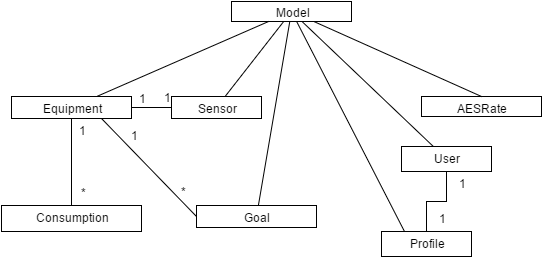
\includegraphics[width=14cm,keepaspectratio]{figuras/diagrama_models.png}
\caption{\label{fig:diagrama-models} Diagrama de Classes - Models}
\end{figure}

No projeto em questão são utilizados Controllers Principais (figura \ref{fig:diagrama-cont-principal}):
\begin{description}
	\item[IndexView:] Exibe página principal sem usuário logado.
	\item[HomeView:] Exibe página principal do usuário logado.
	\item[LoginView:] Exibe formulário para login e realiza autenticação.
	\item[LogoutView:] Encerra a sessão do usuário.
\end{description} 

\begin{figure}[H]
\centering
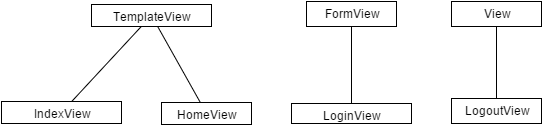
\includegraphics[width=14cm,keepaspectratio]{figuras/diagrama_cont_principal.png}
\caption{\label{fig:diagrama-cont-principal} Diagrama de Classes - Controllers Principais}
\end{figure}

Os Controllers que lidam com os equipamentos estão representados na figura \ref{fig:diagrama-cont-equipment}. E os Controllers são:
\begin{description}
	\item[IndexView:] Exibe página de listagem dos equipamentos.
	\item[CreateView:] Exibe página com formulário para criação de um equipamento, cria um equipamento, realiza redirecionamento após a criação.
	\item[UpdateView:] Exibe página com formulário para edição de um equipamento, edita um equipamento, realiza redirecionamento após a edição.
	\item[DeleteView:] Remove um equipamento.
\end{description} 

\begin{figure}[H]
\centering
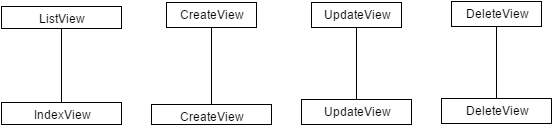
\includegraphics[width=14cm,keepaspectratio]{figuras/diagrama_cont_equipment.png}
\caption{\label{fig:diagrama-cont-equipment} Diagrama de Classes - Controllers de Equipamentos}
\end{figure}

Os Controllers que lidam com os sensores estão representados na figura \ref{fig:diagrama-cont-sensor}. E os Controllers são:
\begin{description}
	\item[IndexView:] Exibe página de listagem dos sensores.
	\item[UpdateView:] Exibe página com formulário para edição de um sensor, edita um sensor, realiza redirecionamento após a edição.
	\item[DeleteView:] Remove um sensor.
\end{description} 

\begin{figure}[H]
\centering
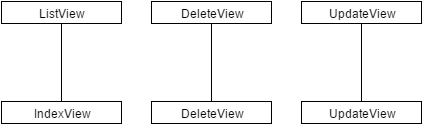
\includegraphics[width=10cm,keepaspectratio]{figuras/diagrama_cont_sensor.png}
\caption{\label{fig:diagrama-cont-sensor} Diagrama de Classes - Controllers de Sensores}
\end{figure}

Os Controllers que lidam com as taxas da AES estão representados na figura \ref{fig:diagrama-cont-aesrate}. E os Controllers são:
\begin{description}
	\item[IndexView:] Exibe página de listagem das taxas AES.
\end{description} 

\begin{figure}[H]
\centering
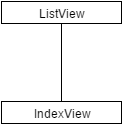
\includegraphics[width=3cm,keepaspectratio]{figuras/diagrama_cont_aesrate.png}
\caption{\label{fig:diagrama-cont-aesrate} Diagrama de Classes - Controllers de Taxas da AES}
\end{figure}

Os Controllers que lidam com as configurações do sistema (e do usuário) estão representados na figura \ref{fig:diagrama-cont-configuration}. E os Controllers são:
\begin{description}
	\item[ConfigView:] Exibe página com formulário para configuração do sistema, configura o sistema.
	\item[UserCreateView:] Exibe página com formulário para registro de um usuário, registra um usuário e realiza redirecionamento após registro.
	\item[UserUpdateView:] Exibe página com formulário para alteração dos dados de um usuário, altera os dados do usuário e realiza redirecionamento após alteração dos dados.
	\item[PasswordUpdateView:] Exibe página com formulário para edição de senha do usuário, edita a senha do usuário e redireciona após a alteração da senha.
	\item[PasswordRecoverView:] Exibe página com formulário para recuperação de senha do usuário, manda e-mail de recuperação de senha.
	\item[PasswordRecoverDoneView:] Redireciona depois do envio de e-mail para recuperação de senha.
	\item[PasswordResetView:] Exibe página com formulário para reconfigurar a senha do usuário, reconfigura a senha do usuário.
	\item[PasswordResetDoneView:] Redireciona depois da reconfiguração de senha do usuário.
\end{description} 

\begin{figure}[H]
\centering
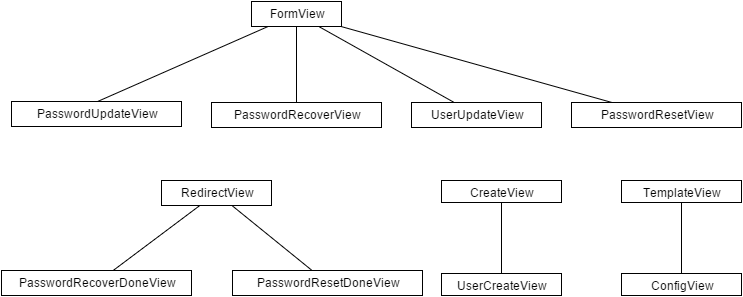
\includegraphics[width=16cm,keepaspectratio]{figuras/diagrama_cont_configuration.png}
\caption{\label{fig:diagrama-cont-configuration} Diagrama de Classes - Controllers de Configuração}
\end{figure}

Os Controllers que lidam com as metas estão representados na figura \ref{fig:diagrama-cont-goal}. E os Controllers são:
\begin{description}
	\item[IndexView:] Exibir página de listagem das metas.
	\item[CreateView:] Exibir página com formulário para criação de uma meta, cria uma meta, realiza redirecionamento após criar a meta.
	\item[UpdateView:] Exibir página com formulário para edição de uma meta, edita a meta, realiza redirecionamento após editar a meta.
	\item[DeleteView:] Remove uma meta.
\end{description} 

\begin{figure}[H]
\centering
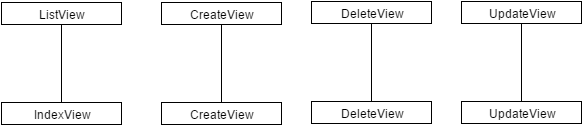
\includegraphics[width=14cm,keepaspectratio]{figuras/diagrama_cont_goal.png}
\caption{\label{fig:diagrama-cont-goal} Diagrama de Classes - Controllers de Metas}
\end{figure}

Os Controllers que lidam com os consumos estão representados na figura \ref{fig:diagrama-cont-consumption}. E os Controllers são:
\begin{description}
	\item[GraphicView:] Exibe o gráfico de consumo
\end{description} 

\begin{figure}[H]
\centering
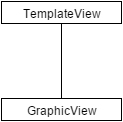
\includegraphics[width=3cm,keepaspectratio]{figuras/diagrama_cont_consumption.png}
\caption{\label{fig:diagrama-cont-consumption} Diagrama de Classes - Controllers de Consumos}
\end{figure}

No mesmo arquivo com os Controllers dos consumos estão localizados os métodos de criação do consumo (a ser chamado quando o Módulo Coordenador enviar uma requisição para a aplicação), importar consumos por arquivo CSV, exportar consumos por arquivo CSV e processar os dados para renderizar através do GraphicView.
\section{Módulo Sensor e Módulo Coordenador}
\label{Sec:5-hardware}

\subsection{XBee: configuração}
Para o projeto em questão, foi usada uma topologia em estrela para a comunicação entre módulos, pois, no caso, existiam poucos componentes no sistema.
O tutorial usado para configurar a rede dos dispositivos XBee encontra-se em \cite{xbee_setup}.

As configurações utilizadas foram: 

\subsubsection{Módulo Sensor:}
\begin{itemize}
	\item Versão de Firmware:
    \begin{itemize}
    	\item Product Family: XB24-ZB
        \item Function Set: ZigBee Router AT
        \item Firmware Version: 22A7
    \end{itemize}
    \item Pad ID: BABABA
        \item Destination Address High: 13A200
        \item Destination Address Low: 40E4429B
        \item Data bits: 8
        \item Baud Rate: 9600
        \item Parity: No parity
        \item Stop Bits: One Stop Bit
\end{itemize}

\subsubsection{Módulo Coordenador:}
\begin{itemize}
	\item Versão de Firmware:
    \begin{itemize}
    	\item Product Family: XB24-ZB
        \item Function Set: ZigBee Coordinator API
        \item Firmware Version: 21A7
    \end{itemize}
    \item Pad ID: BABABA
        \item Destination Address High: 13A200
        \item Destination Address Low: 40E44285
        \item Data bits: 8
        \item Baud Rate: 9600
        \item Parity: No parity
        \item Stop Bits: One Stop Bit
\end{itemize}

\subsection{Raspberry: Sistema Operacional}

Raspberry Pi é um computador, como tal é possível usá-lo com um sistema operacional. O sistema operacional usado é o Raspian, baseado no Debian customizado para rodar no raspberry pi. Apesar de teoricamente não ser necessário o raspberry usar um sistema operacional, facilita muito o desenvolvimento tal equipamento conter uma interface amigável para seu uso.

\subsection{Raspberry: Adaptador Wifi}

Após o sistema Raspian ser instalado no cartão de memória, foi necessário configurar o adaptador Wifi (figura \ref{fig:wifi-adapter}). O modelo usado é o TP-Link TL-WN723N.

\begin{figure}[H]
\centering
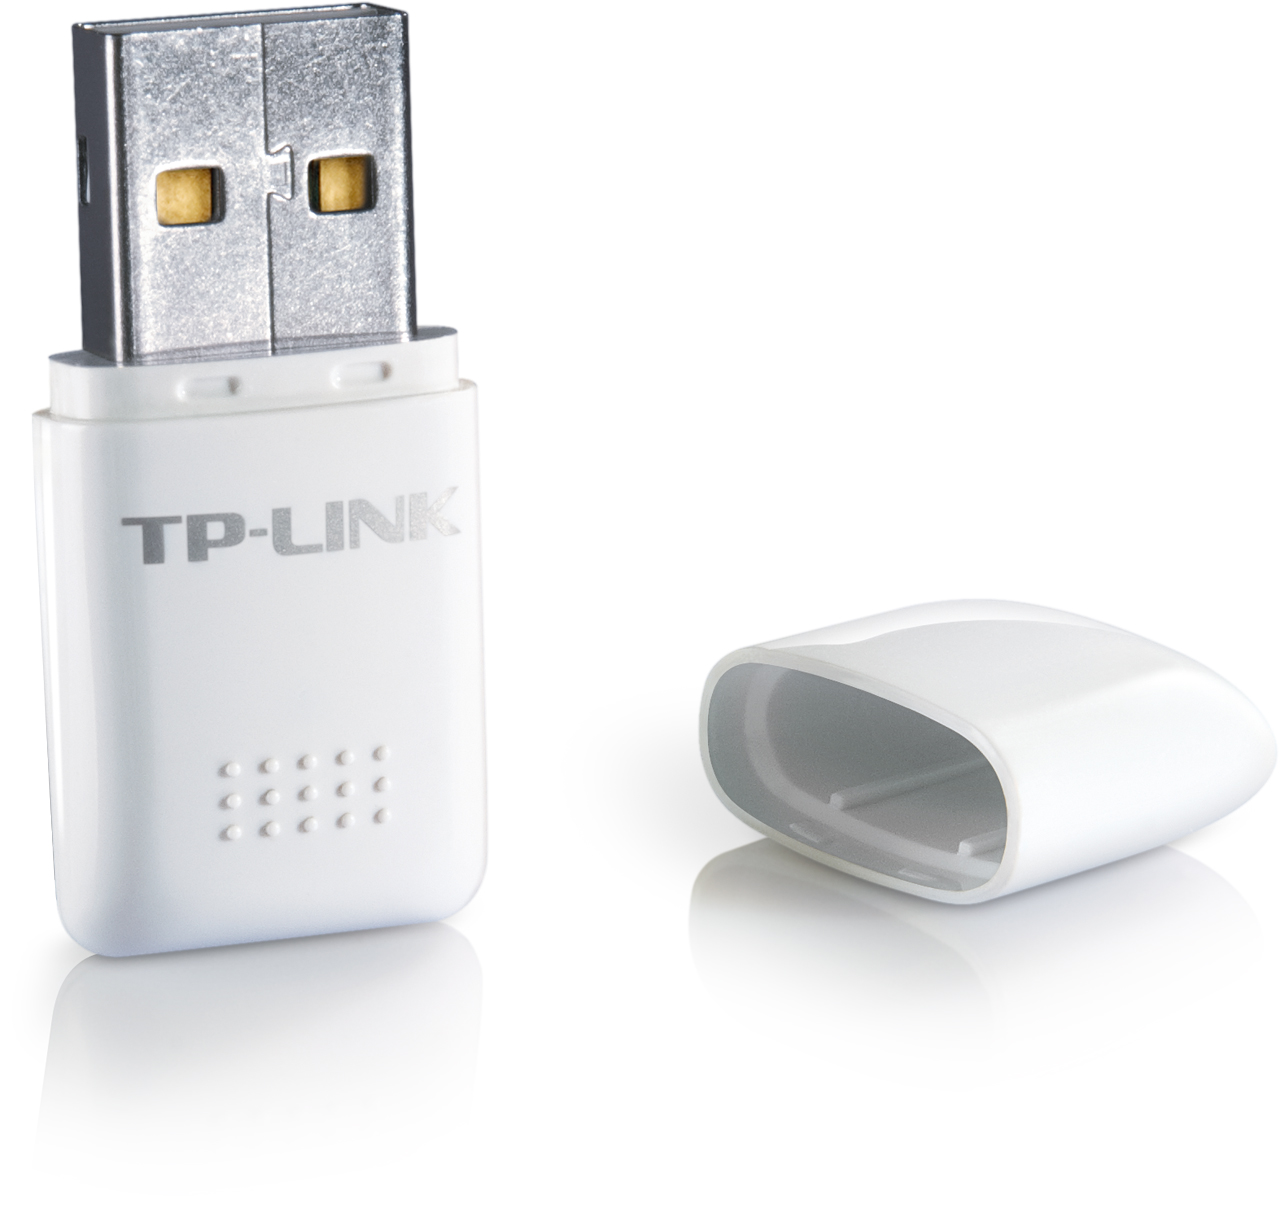
\includegraphics[width=5cm,height=5cm,keepaspectratio]{figuras/wifi-adapter.jpg}
\caption{\label{fig:wifi-adapter} Adaptador wifi usado no raspberry}
\end{figure}

\subsection{Raspberry x Arduino: comunicação}

Para testar a comunicação entre o Módulo Coordenador (figura \ref{fig:teste-inicial-raspberry}) e o módulo sensor (figura \ref{fig:teste-inicial-arduino}), foi montado o esquema representado na figura \ref{fig:teste-inicial-all} e foram executados dois programas: listing \ref{lst:teste-inicial-arduino} e listing \ref{lst:teste-inicial-raspberry}.

\begin{figure}[H]
\centering
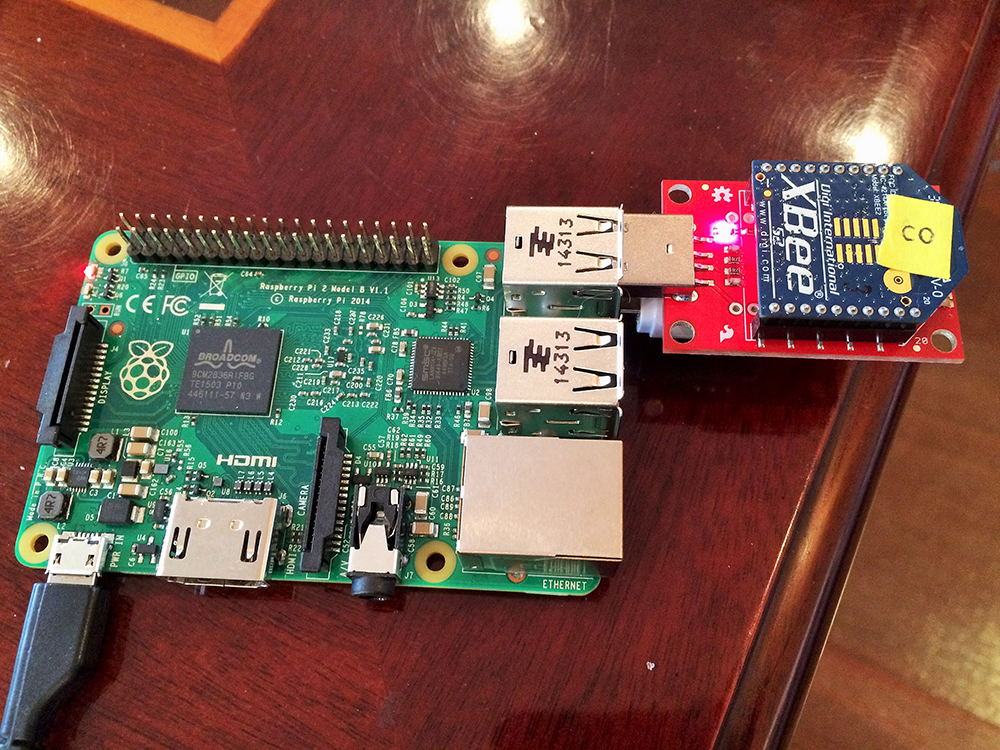
\includegraphics[width=7cm,keepaspectratio]{figuras/teste-inicial-raspberry.jpg}
\caption{\label{fig:teste-inicial-raspberry} Teste de comunicação: Módulo Coordenador}
\end{figure}

\begin{figure}[H]
\centering
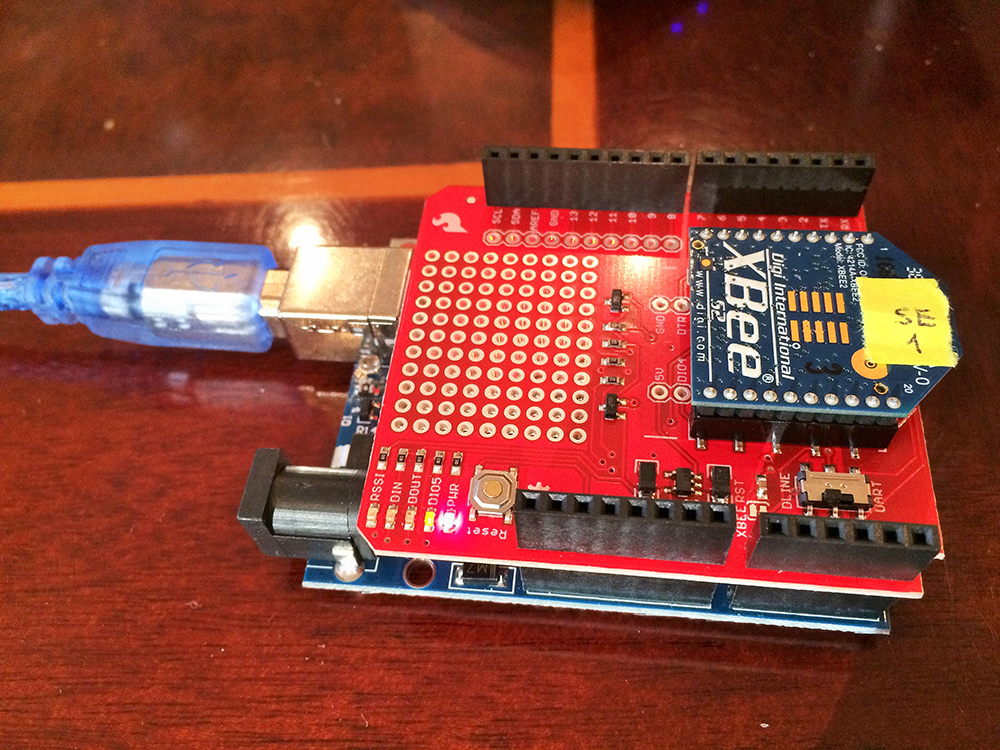
\includegraphics[width=7cm,keepaspectratio]{figuras/teste-inicial-arduino.jpg} 
\caption{\label{fig:teste-inicial-arduino} Teste de comunicação: Módulo Sensor}
\end{figure}

\begin{figure}[H]
\centering
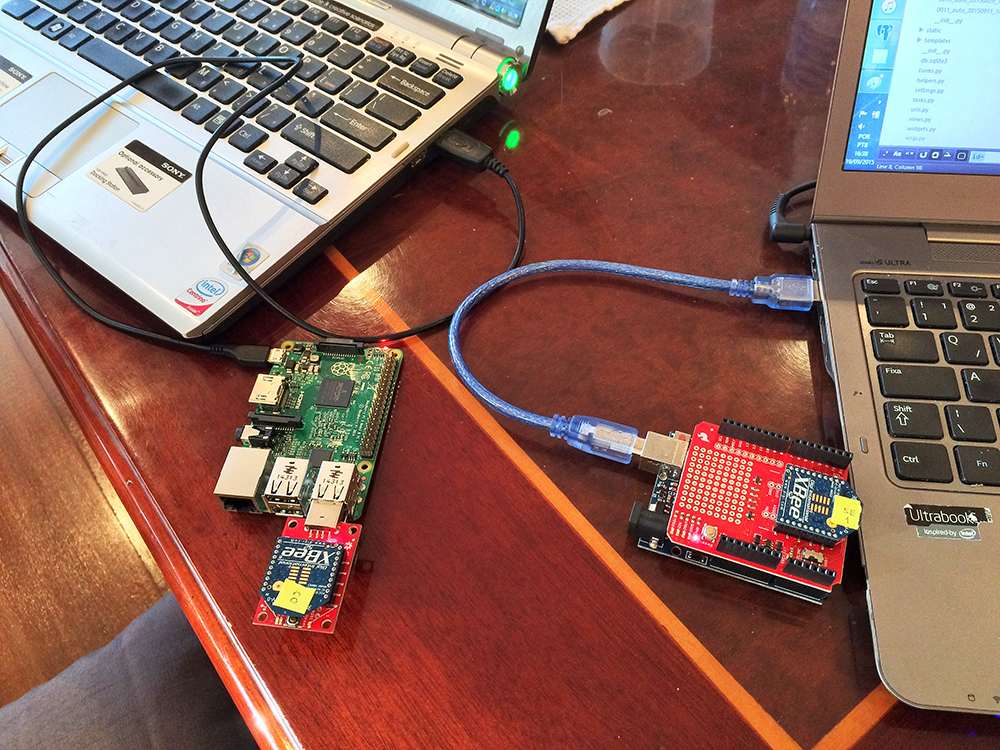
\includegraphics[width=7cm,keepaspectratio]{figuras/teste-inicial-all.jpg} 
\caption{\label{fig:teste-inicial-all} Teste de comunicação: Montagem}
\end{figure}

 O programa listing \ref{lst:teste-inicial-arduino} foi utilizado no módulo sensor para transmitir o valor "123123" por um datagrama a ser enviado pela rede do XBee. Já o programa listing \ref{lst:teste-inicial-raspberry} foi utilizado no Módulo Coordenador para receber o datagrama ZigBee e imprimir no console do Raspberry.

\lstinputlisting[frame=single, language=C, caption=teste-inicial-arduino.c, label={lst:teste-inicial-arduino}]{Anexos/teste-inicial-arduino.c}

\lstinputlisting[frame=single, language=Python, caption=teste-inicial-raspberry.py, label={lst:teste-inicial-raspberry}]{Anexos/teste-inicial-raspberry.py}

Finalmente, na figura \ref{fig:raspberry-arduino-1} é possível observar o resultado do teste: os datagramas que chegavam no raspberry do arduino. No caso, as informações de interesse são ``source\_addr'' que identifica a origem da mensagem e ``rf\_data'', que identifica o valor da mensagem em sí.

\begin{figure}[H]
\centering
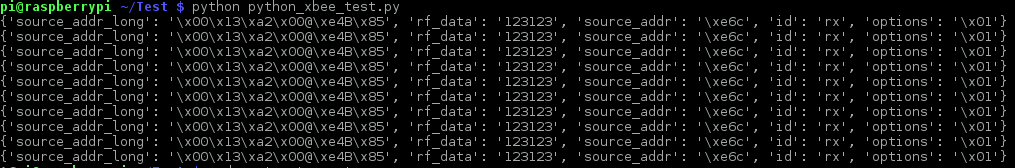
\includegraphics[width=1\textwidth]{figuras/teste-inicial-raspberry-arduino.png}
\caption{\label{fig:raspberry-arduino-1} Teste de comunicação Raspberry e Arduino}
\end{figure}

Após esse teste, foi feito um pequeno teste para observar o que ocorre com multiplos módulos sensores no sistema. Logo, o teste acima foi realizado com dois módulos com frequências diferentes de envio para garantir que não ocorre colisão. Os resultados foram idênticos, com a diferença de que as mensagens chegavam de dois nós diferentes, ou seja, chegavam pacotes com ``source\_addr'' diferentes.

\subsection{Verificador de tensão}

Para verificar a tensão foi usado um transformador para rebaixar a tensão da tomada. Na imagem é possível observar uma tomada de 127V sendo rebaixada para 7,2 V.

\begin{figure}[H]
\centering
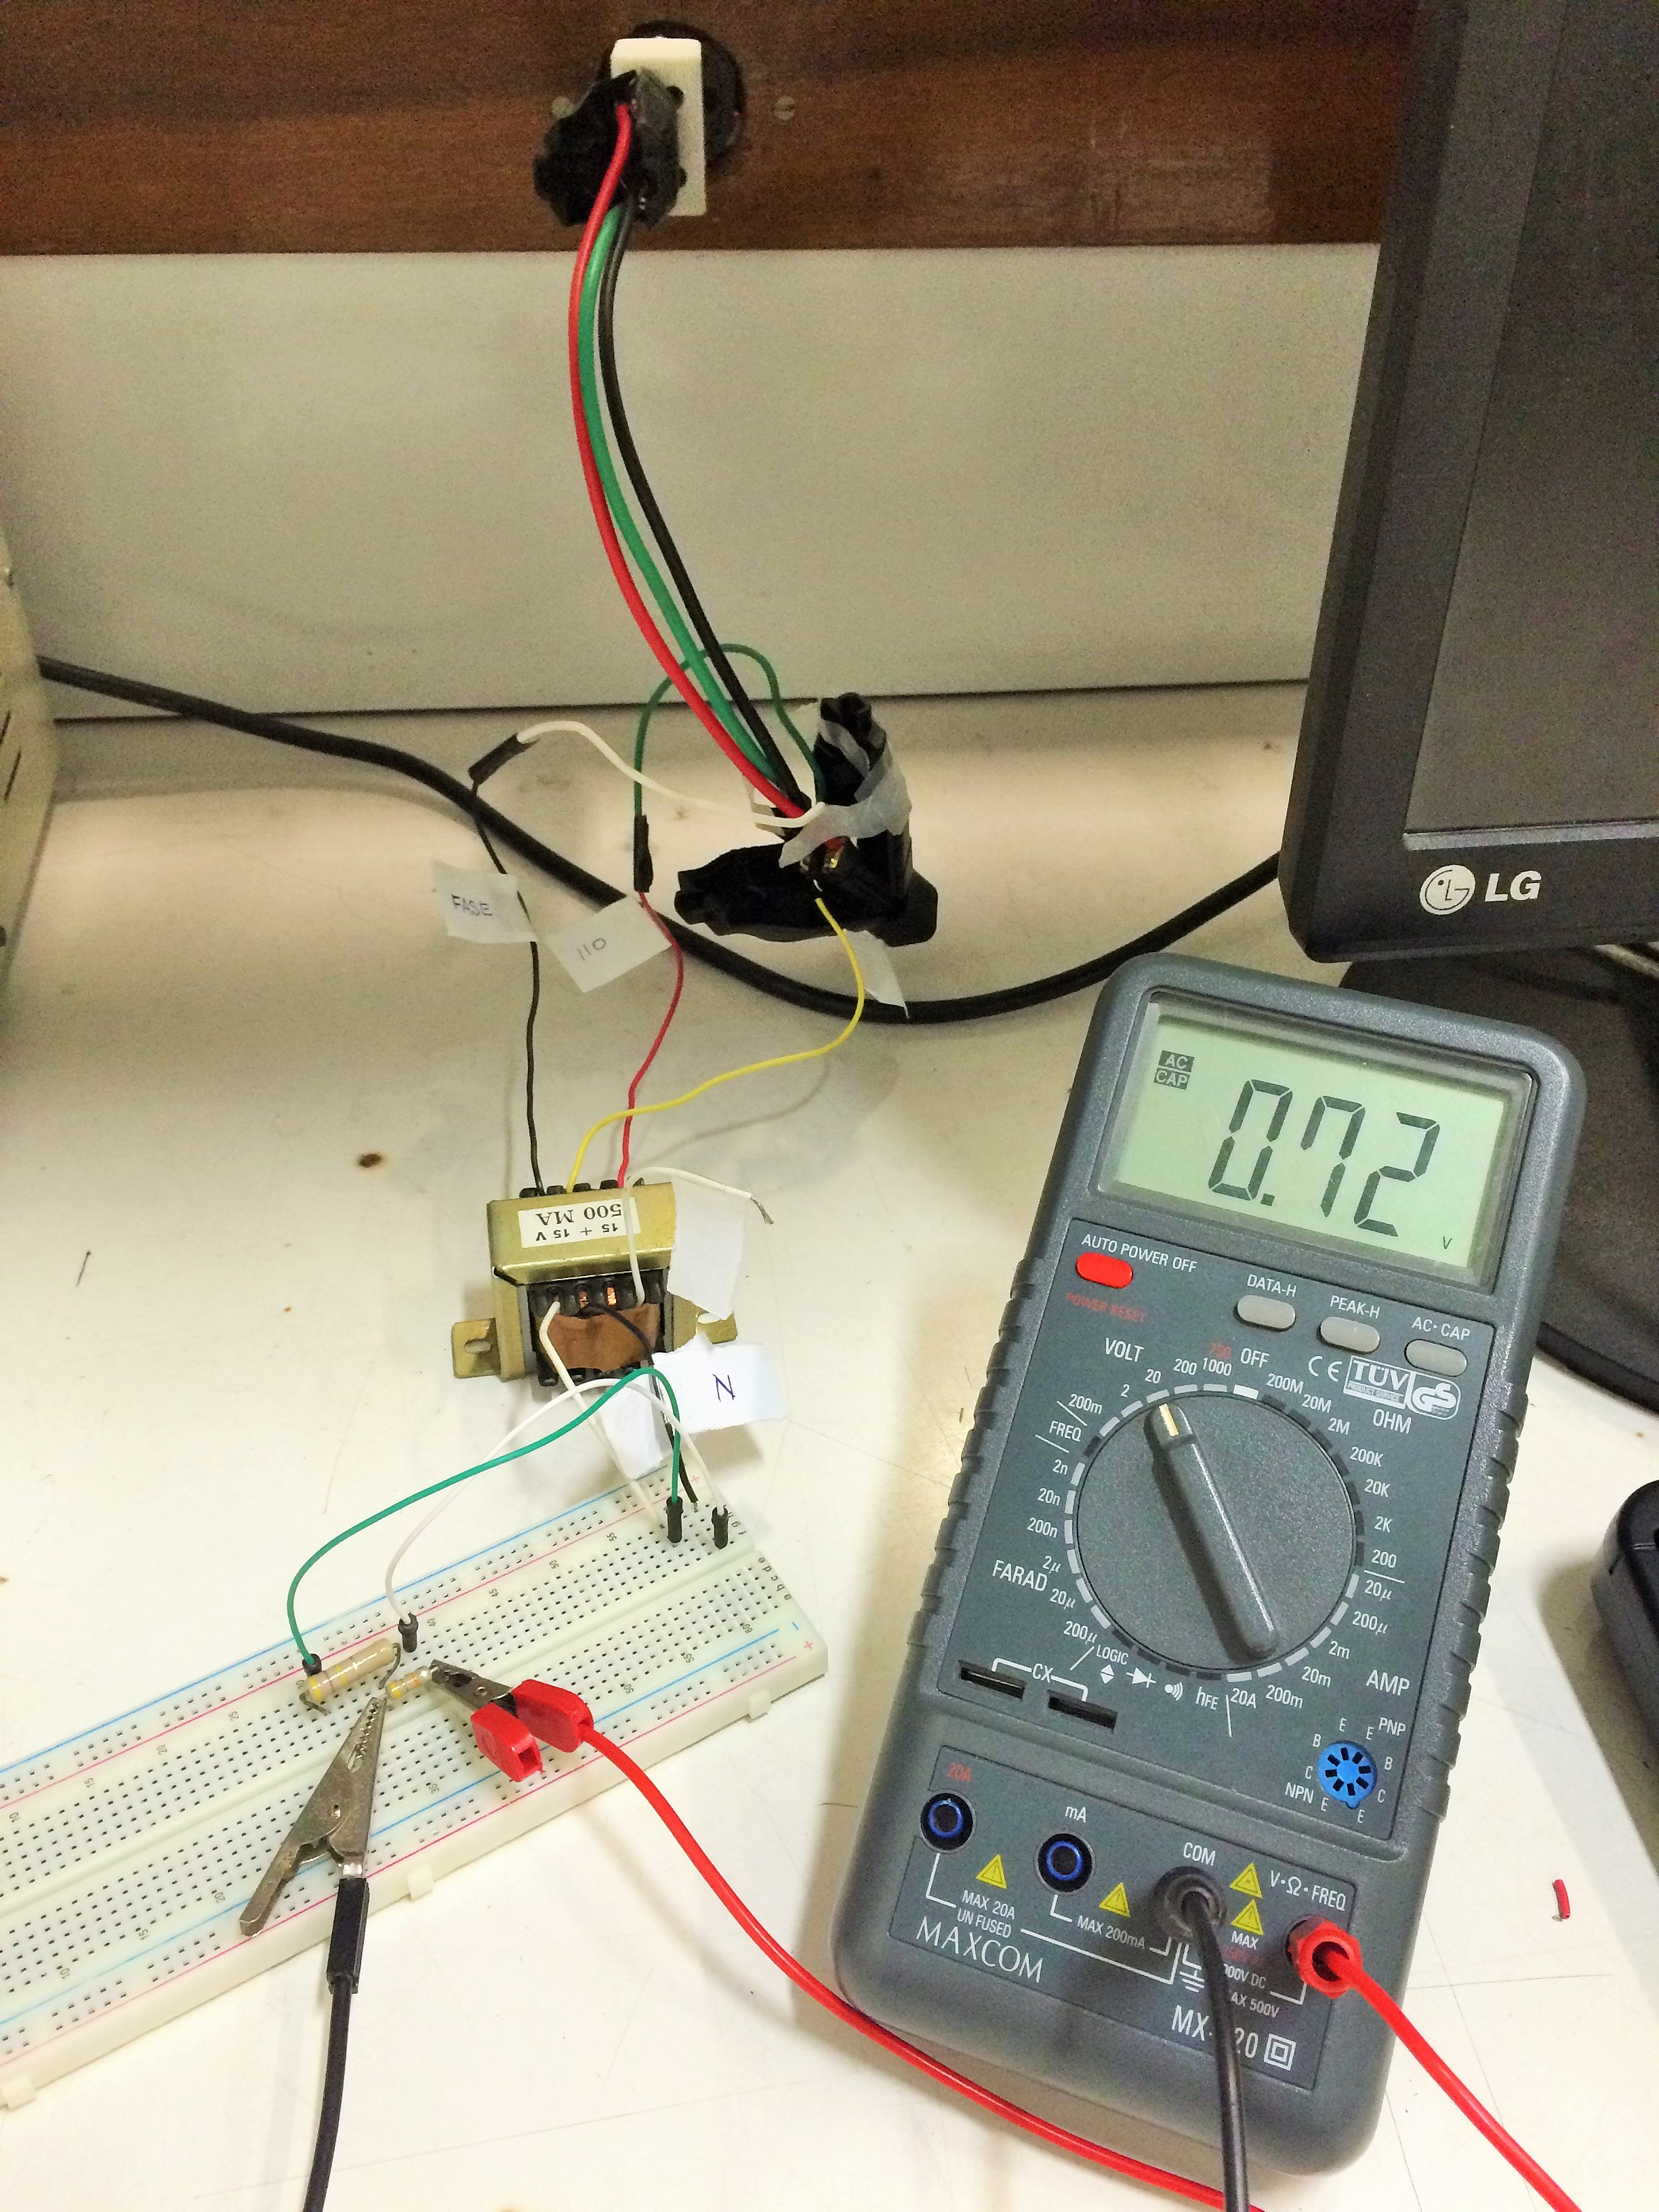
\includegraphics[width=7cm,keepaspectratio]{figuras/sensor-tensao.jpg} 
\caption{\label{fig:sensor-tensao} Teste do transformador}
\end{figure}

Em seguida a saída foi retificada com um retificador de onda completa e filtrada com um capacitor e dividida por divisão de tensão com resistores para que fosse possível diferenciar uma tensão de 220V e 127V no arduino para enviar ao raspberry.

A figura \ref{fig:teste-medicao-voltagem} mostra a montagem para tal e a figura \ref{fig:teste-medicao-voltagem-osc} mostra a saída no osciloscópio.

\begin{figure}[H]
\centering
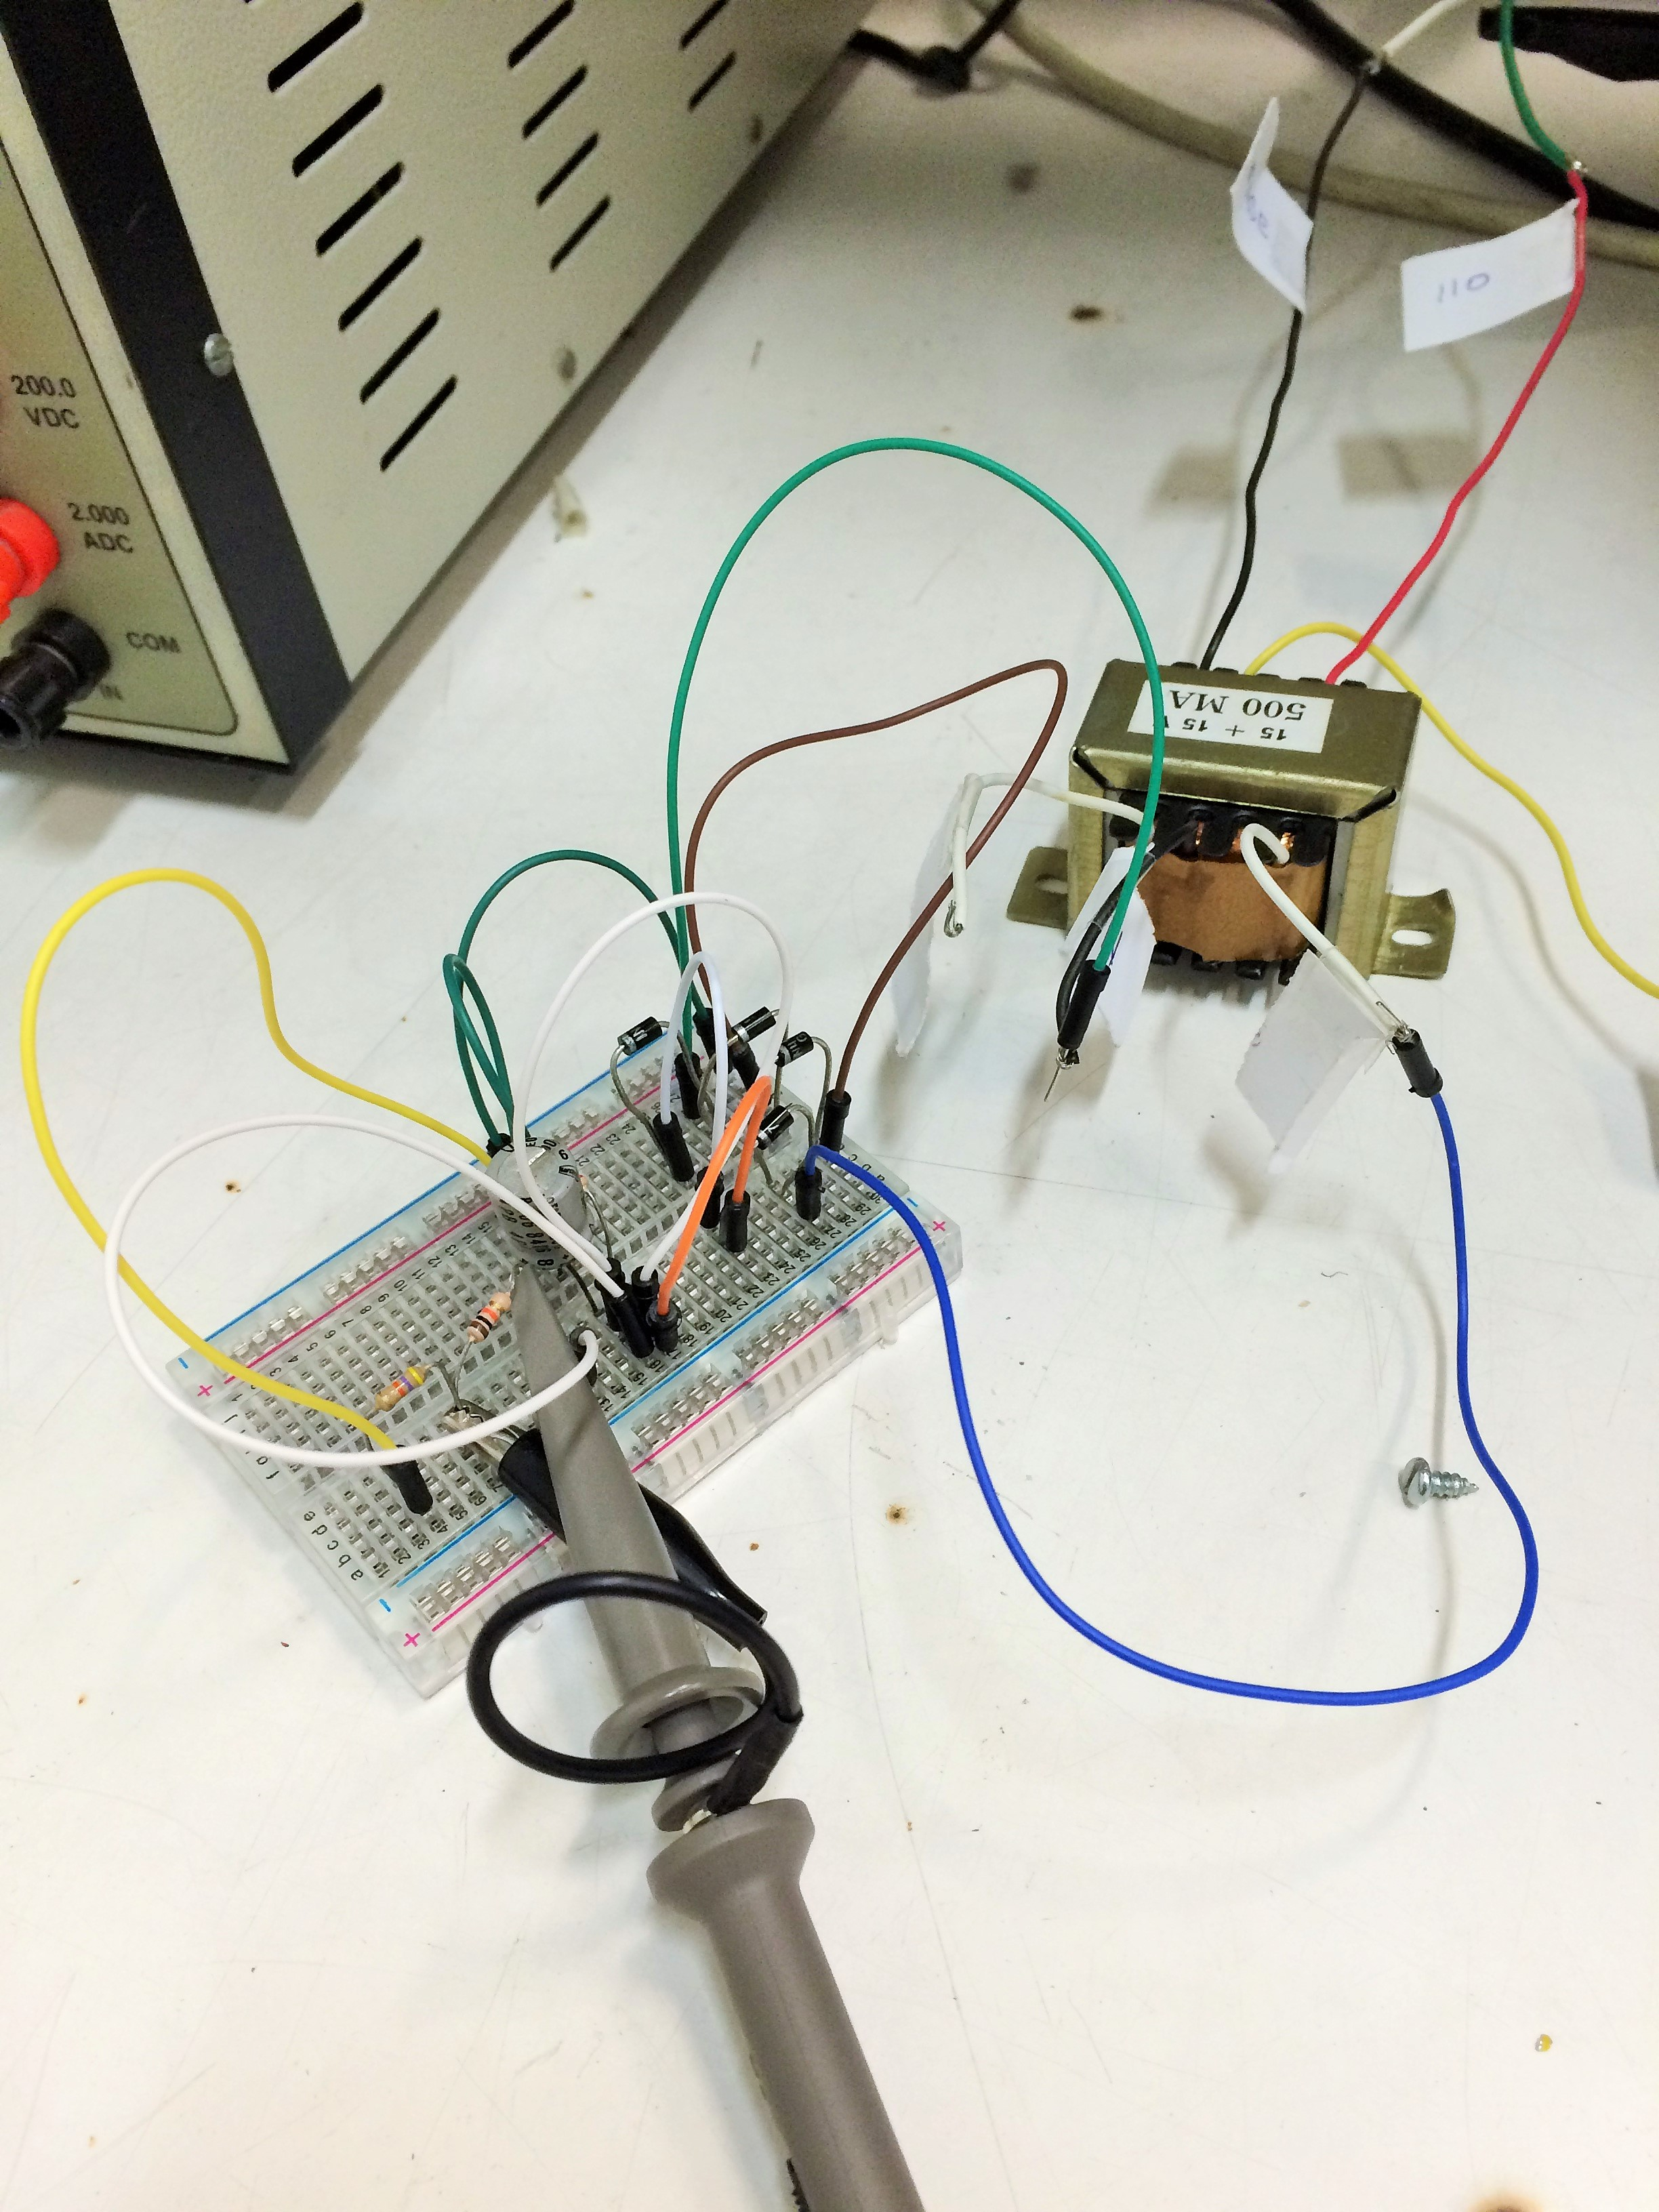
\includegraphics[width=7cm,keepaspectratio]{figuras/teste-medicao-voltagem.jpg} 
\caption{\label{fig:teste-medicao-voltagem} Teste de medição de tensão} 
\end{figure}

Em seguida a saída retificada e dividida foi posta como entrada para um pino de leitura analógica do Arduino para a medição, para 127V e em seguida, 220V. A saída resultante no terminal serial do arduino \ref{fig:teste-medicao-voltagem-osc} foi a seguinte

\begin{figure}[H]
\centering
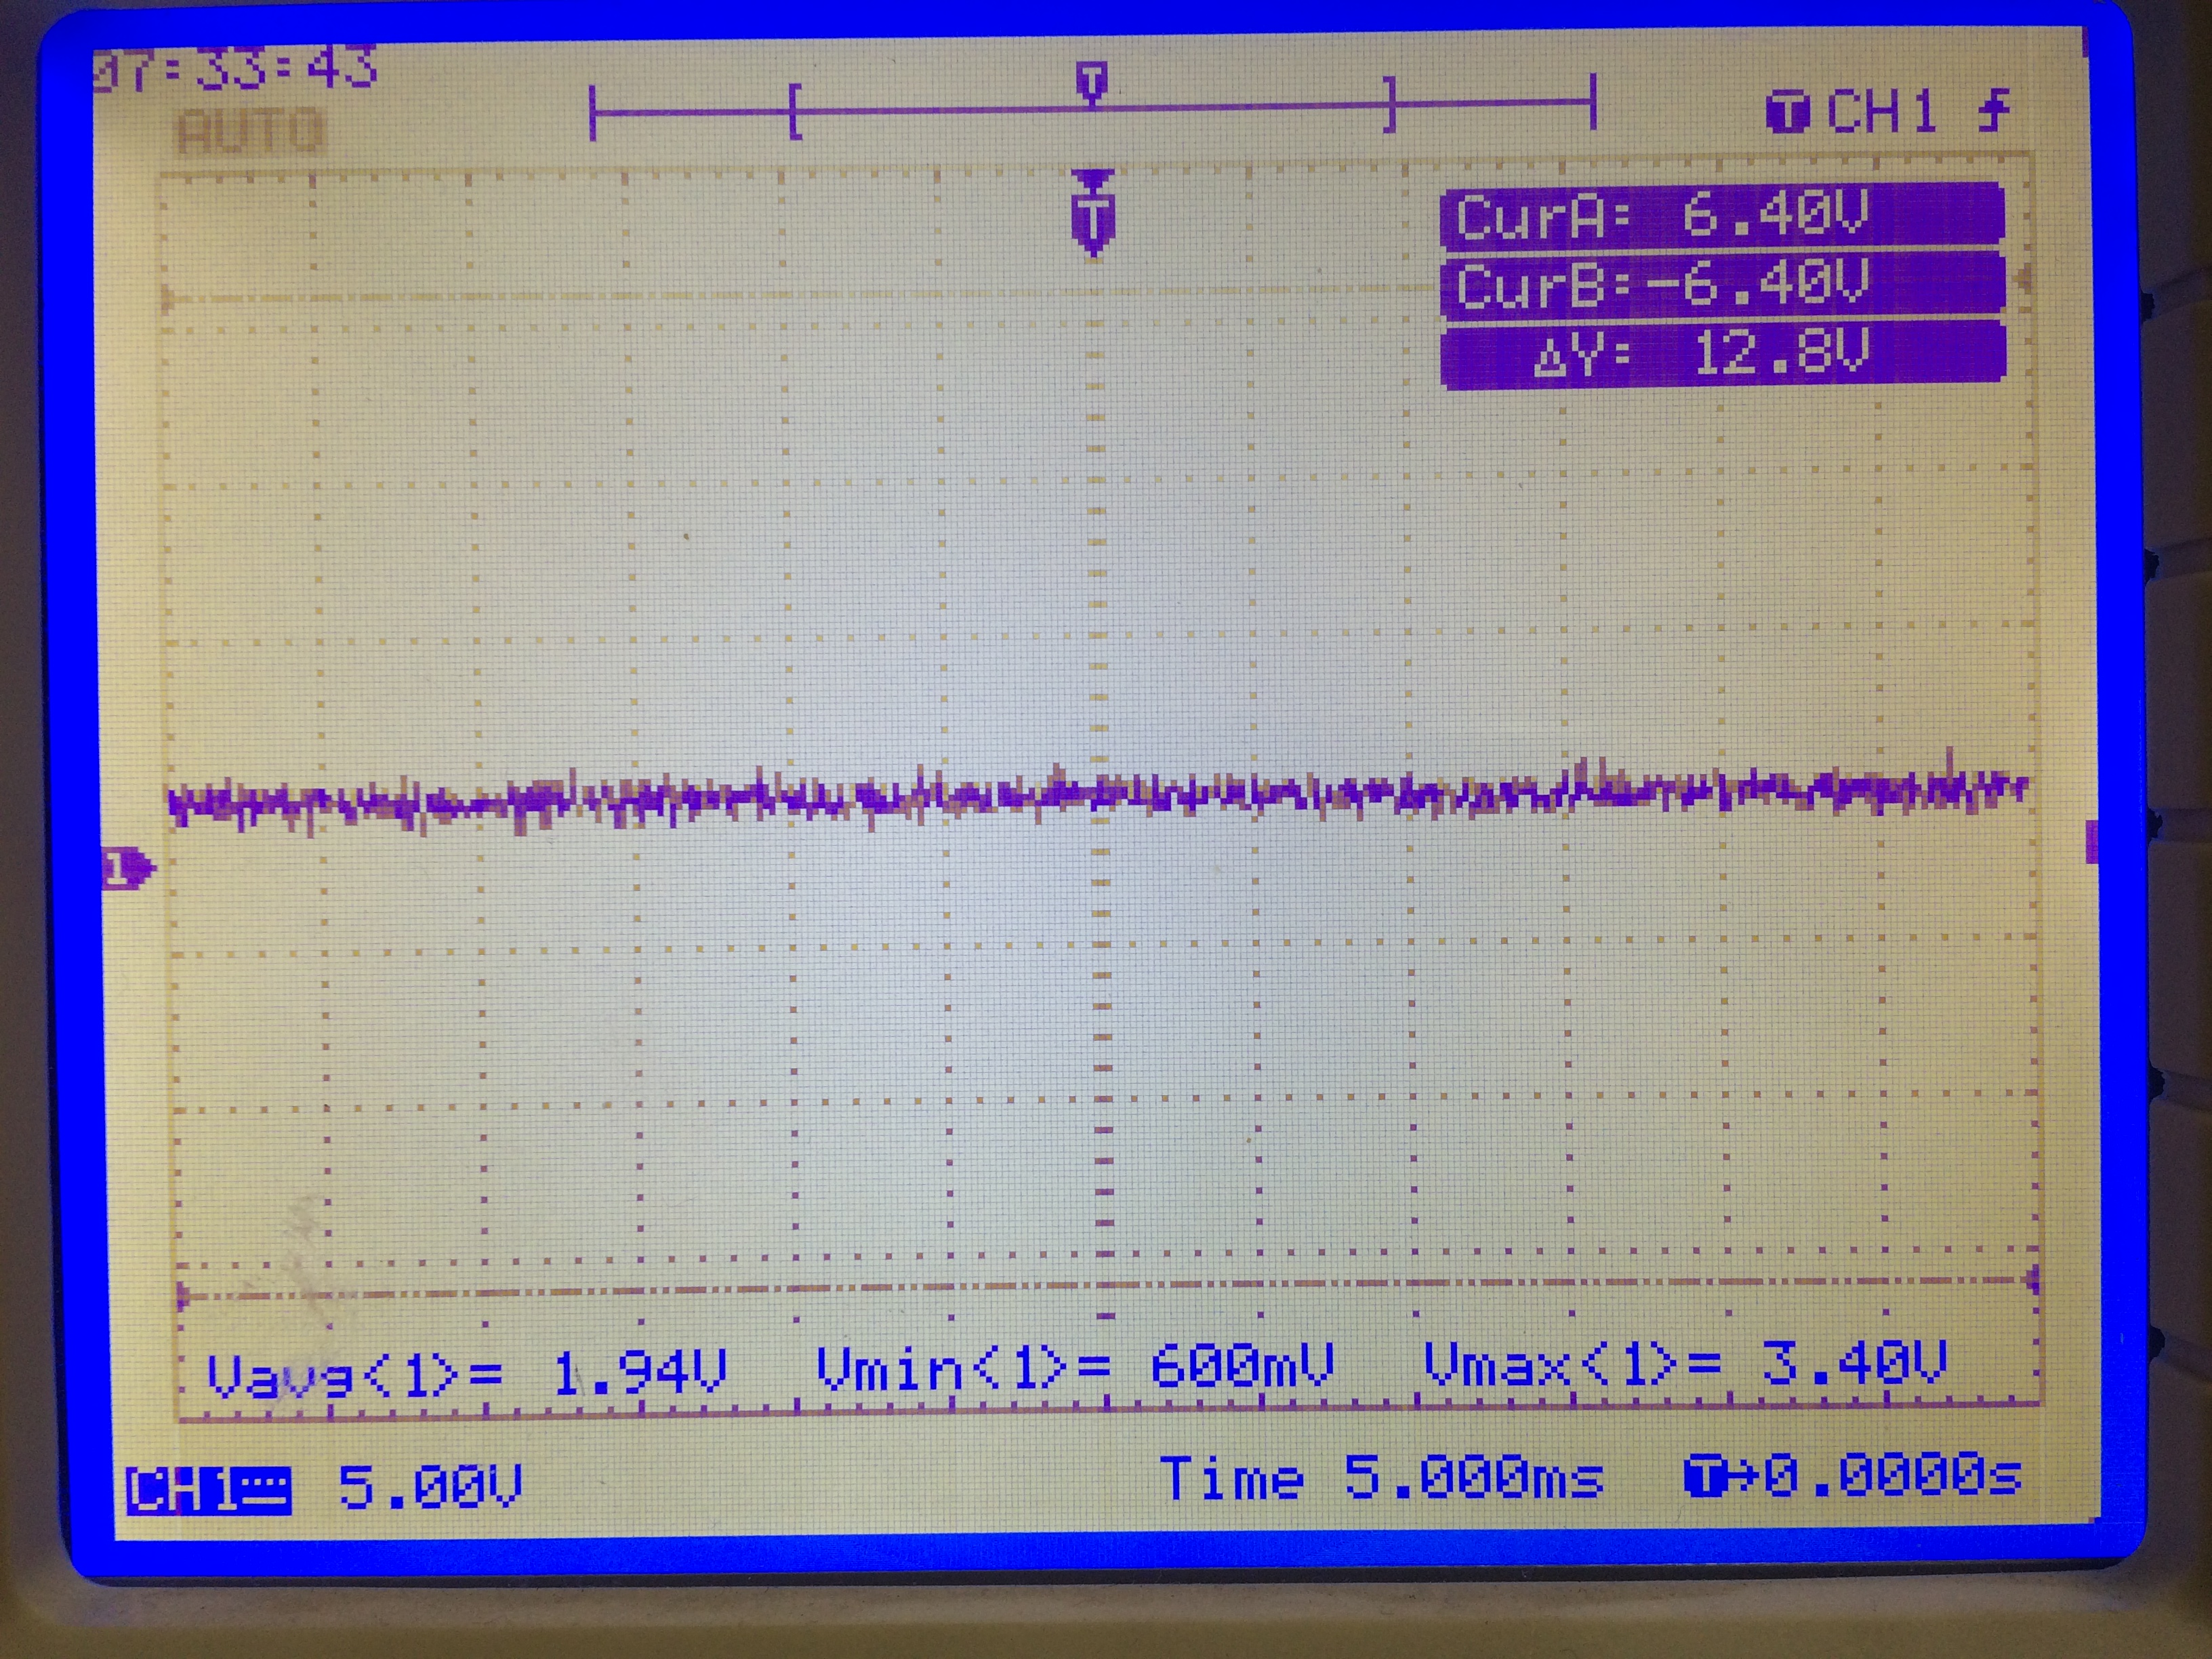
\includegraphics[width=7cm,keepaspectratio]{figuras/teste-medicao-voltagem-osc.jpg} 
\caption{\label{fig:teste-medicao-voltagem-osc} Teste de medição de tensão com arduino - saída do osciloscópio}
\end{figure}

\subsection{Sensor de corrente}

Para o sensor de corrente, dado que a saída do sensor é alternada, foi necessário fazer um pequeno circuito para que as informações coletadas estivessem em uma faixa legível ao arduíno. Para isso, foi colocado uma resistência entre as saídas do sensor, resistência essa que deveria, em 30A (corrente máxima do sensor), resultar em uma tensão máxima de 2,5V para então adicionar um offset de 2,5V, possibilitando amostragens em todos os pontos da onda. Como apenas o valor de pico é relevante para calcular a potência aparente.
No caso, a resistência utilizada foi de 150 omhs. 

Já no arduino, para fazer a leitura, não era possível apenas ler diretamente o valor da entrada analógica, pois estávamos interessados no valor eficaz da corrente. Por isso foi utilizado da raiz da média dos quadrados (tradução livre de RMS - root mean square), fazendo várias leituras sucessivas, assim como o nome do método diz, faz-se a raiz da média dos quadrados das leituras para obter o valor eficaz.

Com o circuito de corrente pronto, foi possível fazer algumas leituras teste. No caso foi usado o ferro de passar para que fosse usada uma corrente mais alta. 

Como se pode ver nos testes, apesar da corrente lida no amperímetro ser 9,3A eficazes (figura \ref{fig:teste-amperimetro}), as leituras no arduíno resultaram em valores ligeiramente menores entre 8,9 e 8,8A eficazes (figura \ref{fig:teste-medicao-corrente-voltagem}), resultando em um erro de aproximadamente 7\%, que é um erro relativamente alto se pensado em uma leitura de longo prazo.

\begin{figure}[H]
\centering
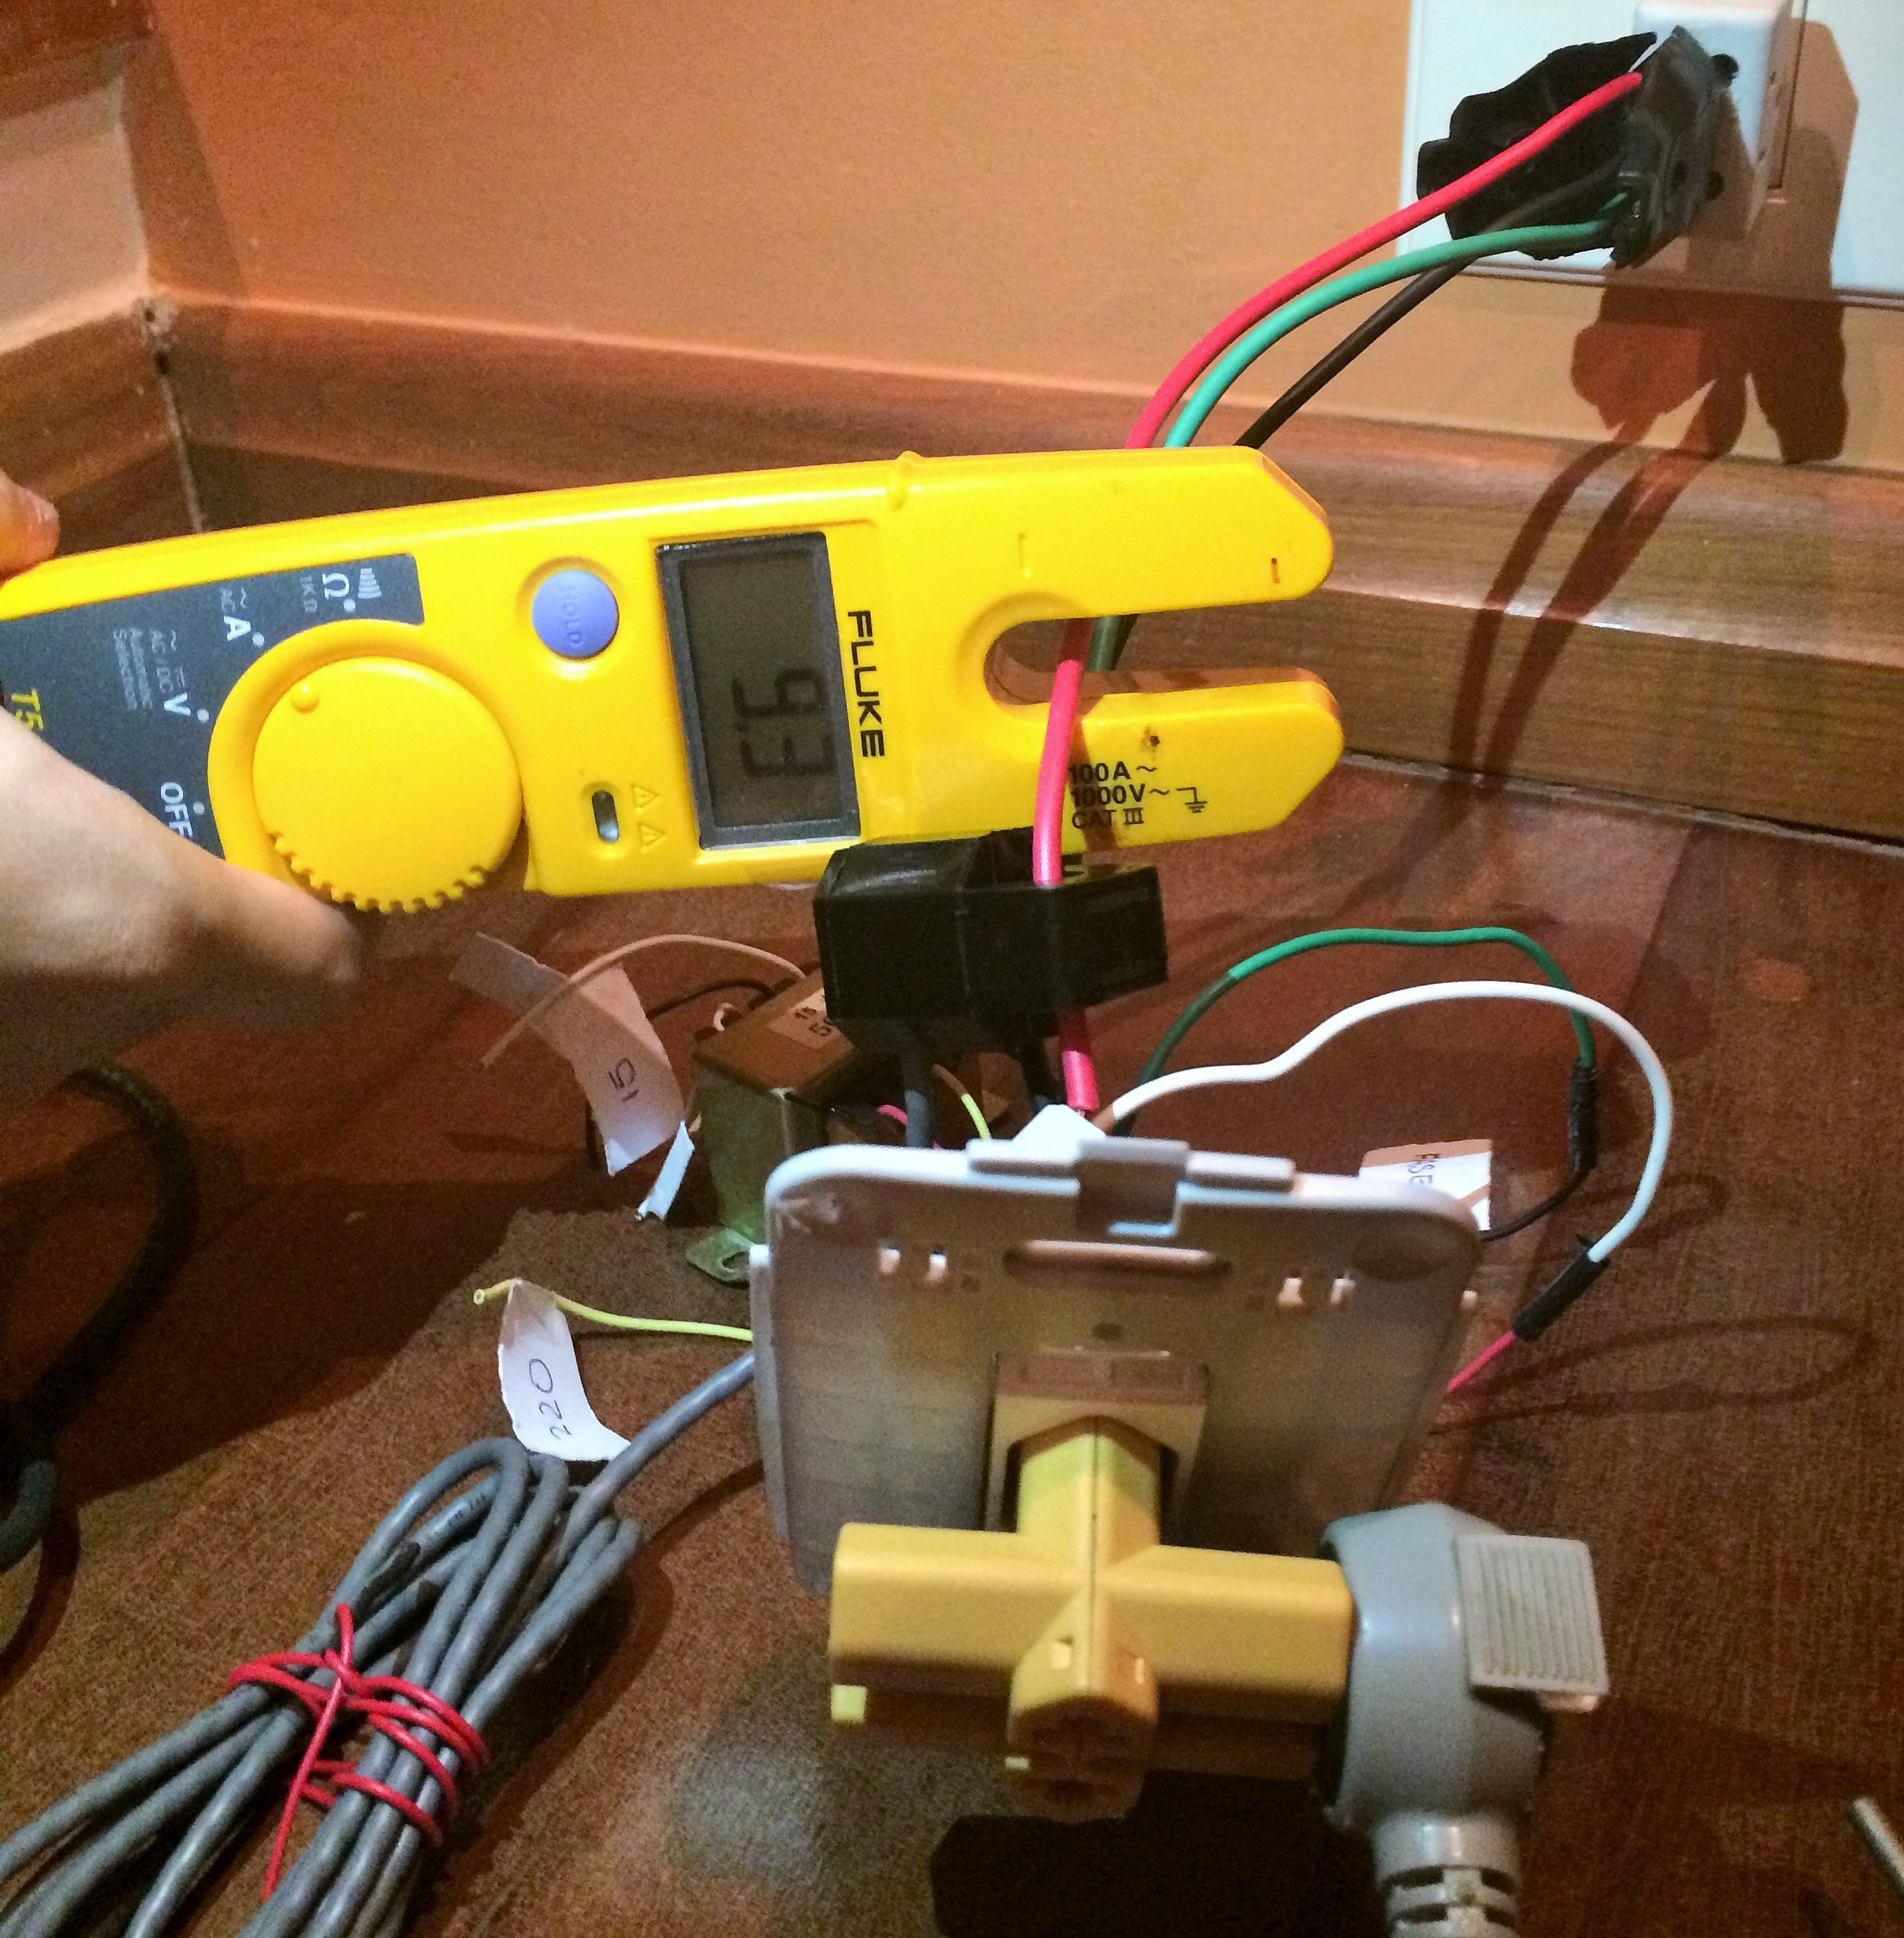
\includegraphics[width=7cm,keepaspectratio]{figuras/ferro-passar-amp.jpg} 
\caption{\label{fig:teste-amperimetro} Medição com amperímetro}
\end{figure}

O código listing \ref{lst:Leitura da corrente} é o código usado no arduino para calcular as medidas.

\lstinputlisting[frame=single, language=C++, caption=Leitura da corrente, label={lst:Leitura da corrente}]{Anexos/voltage_and_current.ino}

Na figura \ref{fig:teste-medicao-corrente-voltagem} aparecem as medidas coletadas no arduino e mostradas no monitor serial da IDE do arduino.

\begin{figure}[H]
\centering
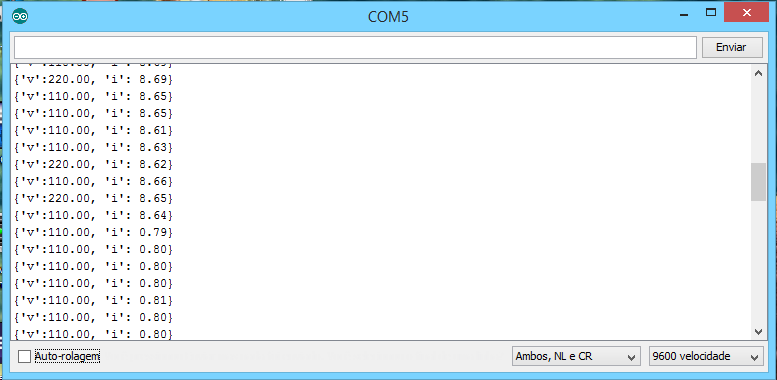
\includegraphics[width=10cm,keepaspectratio]{figuras/ferro-passar.png} 
\caption{\label{fig:teste-medicao-corrente-voltagem} Teste de medição da corrente e tensão}
\end{figure}

\subsection{Integrando as partes}

Após os testes anteriores de comunicação entre o módulo sensor, módulo coordenador e a medição de corrente e tensão, o conjunto foi testado. O código listing \ref{lst:arduino-code} foi carregado no arduino para a coleta dos dados de corrente e tensão e o envio destes para o módulo coordenador.

\lstinputlisting[frame=single, language=C, caption=arduino.c, label={lst:arduino-code}]{Anexos/arduino.c}

O módulo coordenador foi configurado para executar o seguinte programa em python (código listing \ref{lst:raspberry-code}), logo após ligar o raspberry, para a inicialização da interface entre os sensores e a aplicação web. Uma vez com o programa em execução, o módulo coordenador estará pronto para escutar as requisições de envio de dados coletados dos módulos sensores. 

\lstinputlisting[frame=single, language=Python, caption=raspberry.py, label={lst:raspberry-code}]{Anexos/raspberry.py}

A idéia dos códigos é que o arduino envie seu endereço MAC para diferenciá-lo na rede e uma string formatada como um JSON para que esse seja convertido no raspberry e as informações sejam extraídas.

\chapter{Testes e Avaliação}
\label{Cap:testes_avaliacao}

\section{Introdução}
\label{Sec:6-introducao}

Assim como foi especificado pelo grupo no planejamento, foram consideradas duas fases de testes, uma para o software e outra para integração, sendo que na fase de integração também será testado o hardware, uma vez que o hardware não possui nenhuma habilidade de regras de negócio, o foco foi no software que as possui e a integração que era um ponto que envolvia a confirmação da captura dos dados e sua vizualização.

\section{Plano de Testes do Software}
\label{Sec:6-software}

As funcionalidades foram dividídas em funcionalidades críticas e funcionalidades não-críticas. As funcionalidades críticas são aquelas que, caso falhassem, interromperiam o desenvolvimento do projeto e as não-críticas eram funcionalidades que em caso de falha atrapalhariam o desenvolvimento do trabalho, se tornando um incômodo, porém não o interromperiam. Isso ajudou os membros na hora dos testes ao indicar a pessoa fazendo o teste se o teste deveria ser mais intensamente testado ou não. Cada teste é subdivido em testes de falha e teste de sucesso. No teste de falha, o sistema se encarrega de tratar informações ou comportamentos não esperados num fluxo de trabalho normal (ex: submissão de formulário em branco, erro de autenticação, objetos não encontrados no banco de dados, entre outros). No teste de sucesso, o sistema realiza as tarefas esperadas para um fluxo de trabalho normal (ex: submissão de dados válidos num formulário)

\subsection{Funcionalidades Críticas}
\begin{itemize}
\item{realizar login}
\item{visualizar o consumo através de gráficos por equipamento ou total}
\item{Obtenção dos dados da AES eletropaulo}
\item{importar os dados de consumo de um equipamento}
\end{itemize}

\subsection{Funcionalidades Não-Críticas}
\begin{itemize}
\item{exportar os dados de consumo de um equipamento}
\end{itemize}

Com essas funcionalidades categorizadas, foram criados casos de teste para verificar o funcionamento do sistema.

\begin{enumerate}
\item{
  Criação de entidade
}
\item{Leitura de entidade}
\item{Atualização de entidade}
\item{Remoção de entidade}

\end{enumerate}

Feitos esses testes, foi possível descobrir erros, sendo os mais graves na visualização de dados no gráfico e na obtenção de dados do AES devido à mudanças da estrutura do HTML do site, o que impossibilitava a obtenção dos dados, o que mostrou que tal funcionalidade deve ser mantida periodicamente para que tal funcionalidade funcione sempre, pois não é possível prever tais mudanças.
\section{Resultados}
\label{Sec:6-resultados}

Os testes revelaram algumas necessidades adicionais do sistema, como a necessidade de manutenção periódica da aplicação na nuvem, assim como outras imperfeições que limitaram a exatidão do sistema. Porém os resultados foram positivos ao resultar em uma arquitetura escalável e modularizada, o que aumenta as possibilidades do sistema.

\chapter{Considerações Finais}
\label{Cap:consideracoes_finais}

O projeto permitiu o uso dos conhecimentos vistos em aula relacionados à microeletrônica, redes, sistemas digitais, engenharia de software, banco de dados, entre outros. Pelo fato da implementação ter envolvido uma grande variedade de conhecimentos cujas noções básicas foram ensinadas no percorrer da faculdade, o projeto foi muito interessante do ponto de vista de aprendizado, porém dificultou muito a implementação que divergiu um pouco da área de especialização do curso, mas ainda concentrando-se na engenharia.

Ainda relacionado, um grande desafio esteve na parte da implementação dos circuitos, uma vez que o projeto exigia o manuseio direto da rede elétrica, isso deixou os integrantes bem apreensivos, sendo que ao final do projeto o medo foi superado.

O sistema tinha como objetivo prover ao usuário do sistema uma noção do consumo de cada equipamento para que esse tivesse mais controle sobre seus gastos. Além disso, o sistema deveria ser simples de montar e de baixo valor. Pode se dizer que tais objetivos foram alcançados, apesar do alto custo de investimento inicial, sendo que cada equipamento adicional a ser monitorado custaria um adicional de aproximadamente 200 reais (contando o custo do dólar em aproximadamente 4 reais). A teoria envolvida também pode ser considerada simples, dado que hoje em dia há uma diversidade de fontes abertas para o aprendizado. Portanto, o gargalo para a construção do sistema se torna mesmo a vontade que o usuário tem em aprender as técnicas, tecnologias e ferramentas envolvidas e a disponibilidade monetária que esse possui.
\begin{table}
\centering
{\renewcommand{\arraystretch}{1.5}
\renewcommand{\tabcolsep}{0.2cm}
\begin{tabular}{|l|r|r|r|r|r|}
\hline
Componentes & qtd & Total(R\$) & Total(US\$) \\
\hline
XBee 2mW PCB Antenna & 4 & {} & US\$103,80 \\
XBee Explorer Dongle & 1 & {} & US\$24,95 \\
Kit Raspberry Pi2 & 1 & R\$309,89 & {} \\
Sensores de Corrente & 3 & {} & US\$29,85 \\
XBee Shield & 3 & {} & US\$44,85 \\
Arduino Stackable Header Kit & 4 & {} & US\$6,00 \\
Arduino Uno - R3 & 3 & R\$ 137,70 & {} \\
\hline
\multicolumn{2}{|l|}{Totais} & R\$447,59 & US\$209,45 \\
\hline
\end{tabular}}
\caption{\label{tab:orcamento} Orçamento das peças necessárias.}
\end{table}

\bibliographystyle{plain}
\nocite{*}
\bibliography{bibliografia}

\end{document}